\documentclass[10pt,letterpaper]{article}
\usepackage[latin1]{inputenc}
\usepackage{amsmath}
\usepackage{amsfonts}
\usepackage{amssymb}
\usepackage{graphicx}
\usepackage[left=3.00cm, right=3.00cm, top=4.00cm, bottom=4.00cm]{geometry}

\title{\textbf{User Guide for\\ Multicopter Design 0.2}}

\author{Tao Du\\taodu@csail.mit.edu
\and
Adriana Schulz\\aschulz@csail.mit.edu
\and
Bo Zhu\\boolzhu@csail.mit.edu}
\date{MIT Computer Science and Artificial Intelligence Laboratory}

% Forcing a floating image to be at the top when it is the only element in a page.
\makeatletter
\setlength{\@fptop}{0pt}
\makeatother

\begin{document}

\maketitle

\tableofcontents

\clearpage
\section{Introduction}\label{sec:intro}
This project is about developing a design, simulation and optimization tool for casual users to build their own multicopters. Initially it was a research project led by the Computational Fabrication Group at MIT CSAIL in 2015. After we published a paper~\cite{du2016} we got inquiries from many different sources so we decided to release our source code for the benefits of both the research and hobbyist communities.

For those who have read that paper, please note that the code here only covers a subset of our implementation in the paper, as we are still in the middle of cleaning it up. We expect to release all features in the next version ($0.3$).

\subsection{Problem Definition}
Suppose you are a drone hobbyist who wants to have more fun in building your own copters. Below is a list of questions you might want to ask yourself before you start:
\begin{itemize}
\item What components to use: This includes choosing the right material to build the frame (carbon fiber, wood, plastic, etc), picking the proper motors and propellers, selecting a good battery, and many more.

\item How to assemble them: You may want to follow standard designs like a quadcopter, or try some fancy configurations like a tricopter, or even come up with your own, unique configuration, like the bunny-shaped example in our paper.

\item How to control its flight: Normally, you can find a mature controller design for classic quadcopters, which is typically a multi-layer PID controller, for example. If you want to have more degrees of freedom in our design, you probably need to develop your own controllers, or at least spend some time modifying and tweaking an existing controller from similar models.

\item How to verify the design: Crashing a real drone is a huge pain and loss, both psychologically and financially. This is why people turn to software simulation for help. Ideally, it should verify both the geometry and controller accurately, and it should be embedded in the design loop to allow for interactive changes.
\end{itemize}
Obviously, this is a very involved process requiring a diverse set of skills, including mechanical engineering, electrical engineering, programming, control theory, and hands-on experience in building stuff. The goal of our software is to expedite and simplify this process by hiding low level technical details so that people can focus more on expressing and exploring the design space. Specifically, we provide:
\begin{itemize}
\item A dataset of standard components that users can freely choose from and assemble by defining their own scripts.
\item An easy-to-use user interface to explore designs in an interactive way.
\item An automatically determined LQR controller that is generalizable for most existing designs we have seen so far.
\item A real-time simulation tool seamlessly embedded in the design loop to visualize results instantly.
\end{itemize}

Please keep in mind that this software is not meant to replace all the work involved in building a customized drone. You are expected to do your own measurement, or at least give a rough estimation of the physical properties of the motors, propellers and batteries. The output of our software is a hardware specification you can follow, but of course you still need to fabricate or buy these components and assemble them manually. Finally, we include a controller in the solution, but uploading it into your own flight controller board is beyond the scope of this software. You are expected to have a working knowledge of the flight controller (both the hardware and software) you plan to use, and be comfortable with modifying its code to include a new controller.

\subsection{Inputs and Outputs}
The input is an XML file that defines the initial copter design. It provides a straightforward way to format all the essential information needed in the software. We provide a few sample XML files for you to start with, including a standard quadcopter, a V-Tail quadcopter, a Y6 hexacopter and a ``pentacopter'' with 5 motors. Section~\ref{sec:file} provides a detailed explanation on the file format for your reference.

The output includes a hardware fabrication plan and a matrix of control parameters. This plan provides hardware specifications like rotor positions and tube sizes so that by following it you should be able to replicate your virtual design. The control parameters fully determine the LQR controller, and if you are familiar with your flight software it should be fairly straightforward to translate them into the code on board.

\subsection{An Example}
As a concrete example, here we demonstrate how our software can be used to help design and simulate a V-Tail copter~\ref{fig:vtail_ui}. When the window first pop up, you will see a V-Tail model centered on screen, and a few windows floating on both sides. Below we will briefly explain the user interface and show a simple design and simulation loop. A more thorough description can be found in Section~\ref{sec:ui}.
\begin{figure}[!htb]
  \centering
  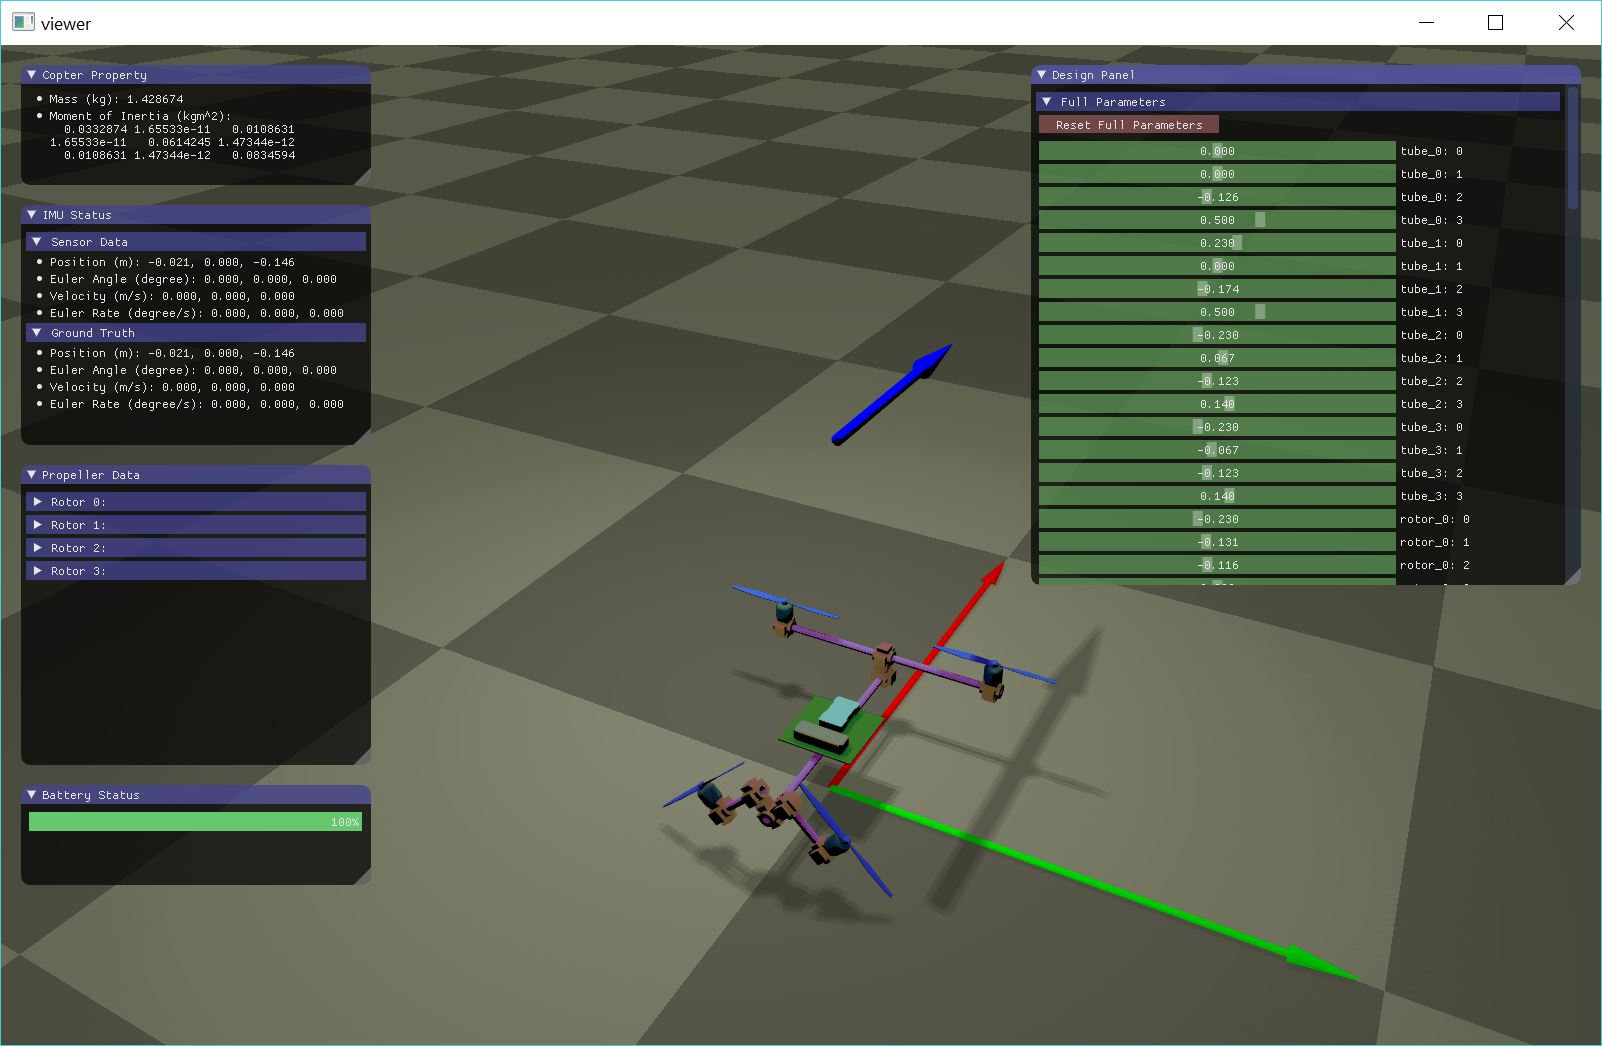
\includegraphics[width=0.9\linewidth]{vtail_ui}
  \caption{Loading the given V-Tail design into our software. The left windows show the current status of the copter, and the right panel allows you to freely explore and simulate different designs.}
  \label{fig:vtail_ui}
\end{figure}

\subsubsection{Basic Information}
On the top left you will find a window named ``Copter Property''. This consists of the mass and inertia of the current design, both of which are computed by collecting information from each component in the XML file. Later, when you change your design, this panel will get updated automatically.

\subsubsection{Design Panel}
On the right there is a long window for you to explore more design possibilities. In our software a copter is parametrized, meaning its shape is fully determined by a list of underlying parameters. These include the length of a tube, 3D position of a connector, height of a plate, and so on. Certain constraints are imposed to ensure the parameters are feasible. For example, a motor should always be attached to a connector instead of freely floating in the air. Please refer to Section~\ref{sec:file} for more details about parameters in each component and its constraints.

\paragraph{Full Parameters} The first panel named ``Full Parameters'' lists a union of parameters from each component. When you use a slider, it specifies a desired value of that particular parameter. A linear least square problem is then solved to find parameters that respect all constraints and are closest to the desired value. Once a solution is found, the copter design in the middle gets updated automatically, and usually in real time (Figure~\ref{fig:vtail_change_full_param}).
\begin{figure}[!htb]
  \centering
  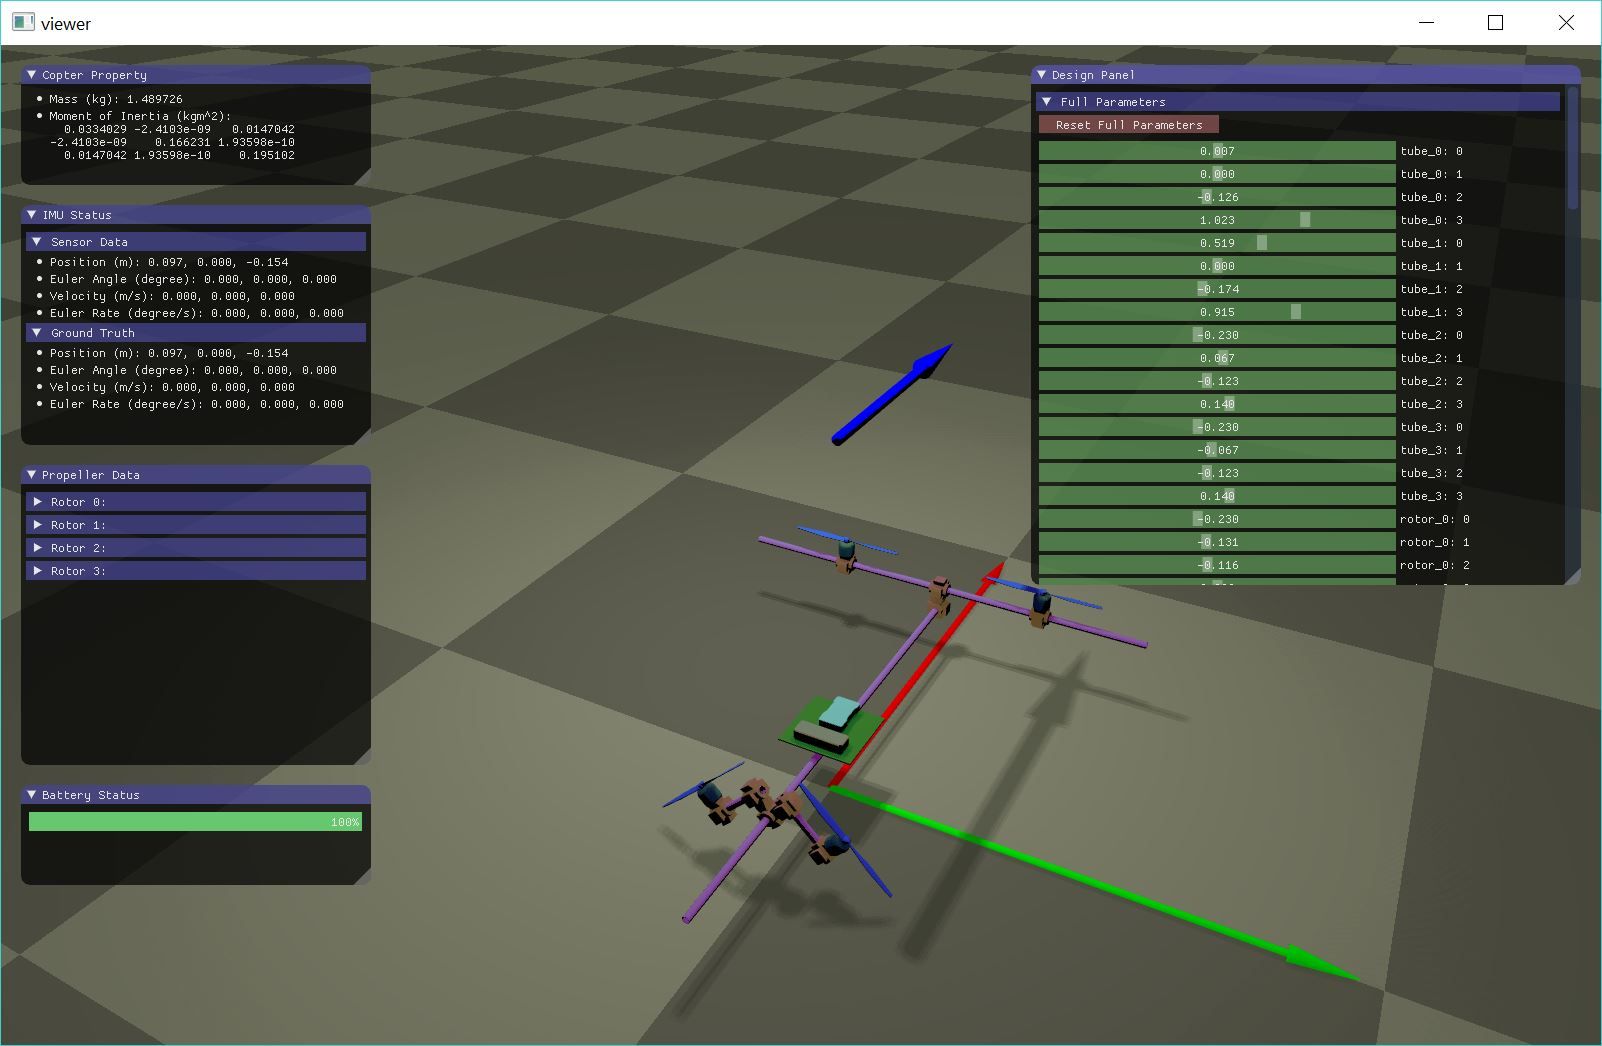
\includegraphics[width=0.9\linewidth]{vtail_change_full_param}
  \caption{By adjusting the full parameters, we elongate two tubes and push the front rotors farther from the center.}
  \label{fig:vtail_change_full_param}
\end{figure}

\paragraph{Reduced Parameters} A copter design consists of up to hundreds of parameters. However, most of them are over constrained by the relative locations between different components. As a result, we also provide a panel to manipulate the reduced parameters, which is usually less intuitive but has way fewer degrees of freedom. Technically, this is done by replacing the linear equality constraints with vectors in its null space.

When you slide the reduced parameters, you may notice the background color sometimes changes between green and red. This color indicates the current parameter is feasible (green) or breaks certain constraints (red). If you slide it into red, the new value will be rejected and the current design remains unchanged.

Finally, there is a ``Reset'' button in both ``Full Parameters'' and ``Reduced Parameters'' windows. Simply clicking it will reset the copter to its original design.

\subsubsection{Simulation}
Once you are satisfied with the current copter, scroll down in the design panel, and you will find a ``Simulate'' button. Clicking it will trigger the software to compute a proper LQR controller and start simulating a virtual flight (Figure~\ref{fig:vtail_simulate}). Press this button will invalidate the ``Full Parameters'' and ``Reduced Parameters'' windows. The button itself will change to ``Reset'' so that you can switch back to the design process if more iterations are needed.
\begin{figure}[!htb]
  \centering
  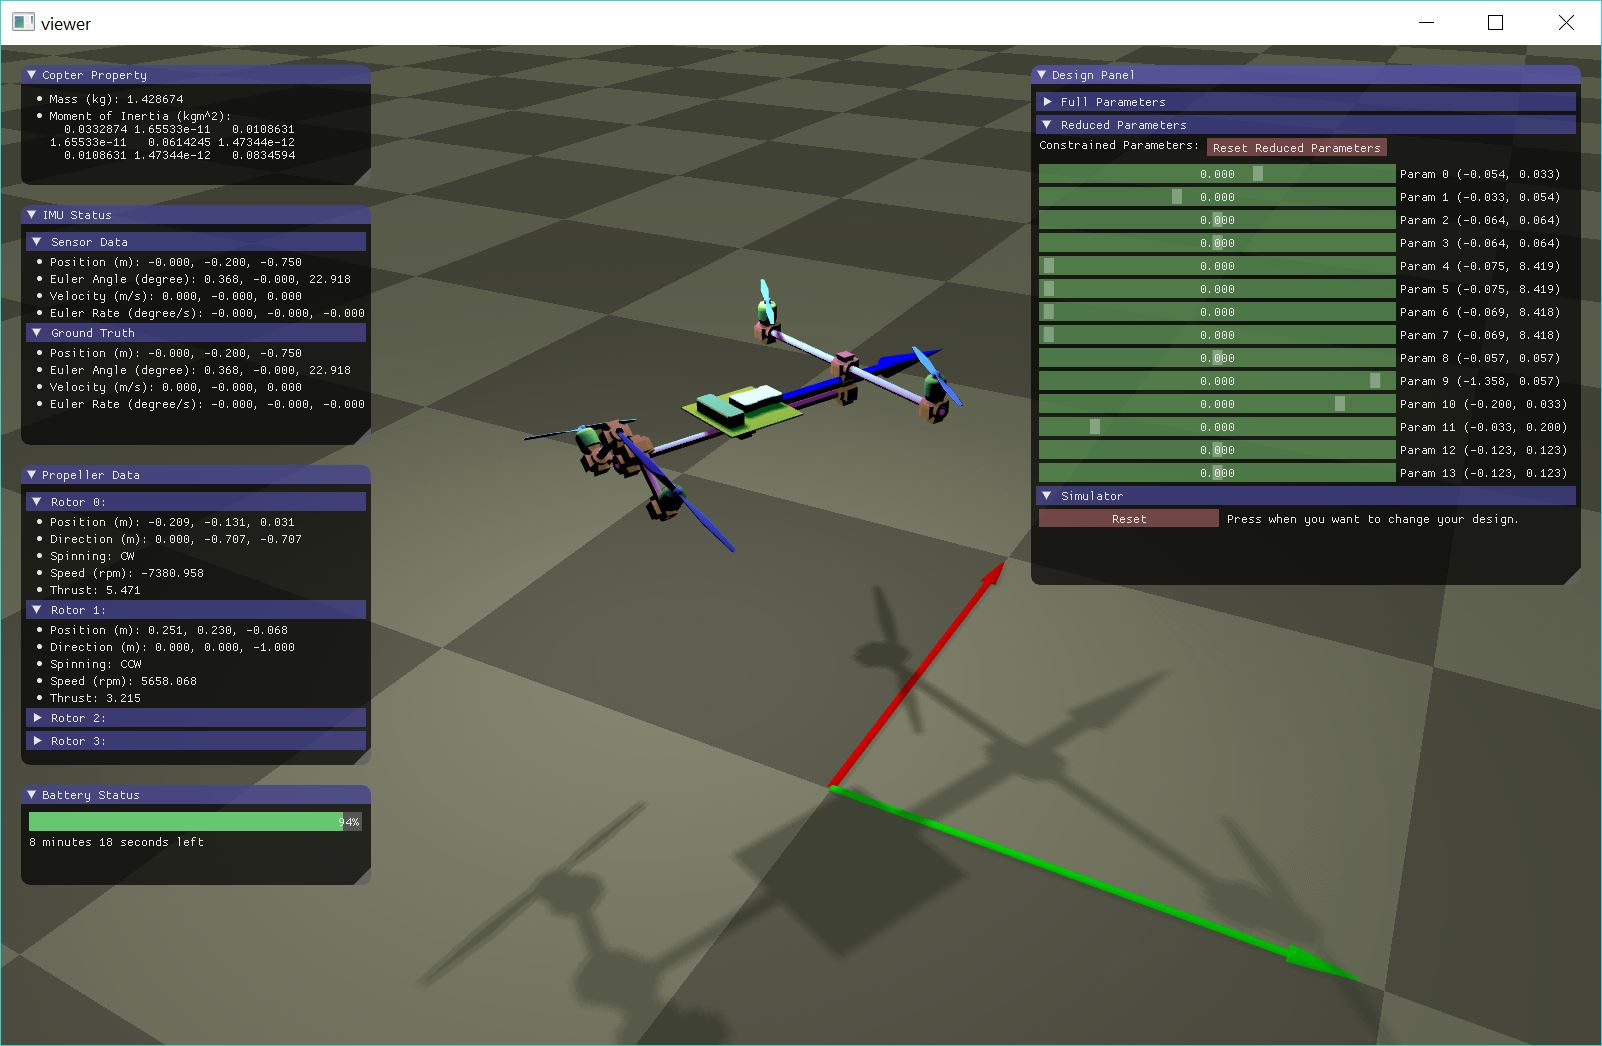
\includegraphics[width=0.9\linewidth]{vtail_simulate}
  \caption{The V-Tail quad is executing a virtual flight in simulation. The copter is trying to follow the position and heading specified by the blue arrow.}
  \label{fig:vtail_simulate}
\end{figure}

During the flight, this copter will try to track the blue arrow as close as possible. Specifically, it interprets the tail as the target position and the arrow as the desired heading. You can use the four arrow keys plus `a', `d', `w' and `s' to adjust the blue arrow and guide your copter to a desired position. You can also change the camera view by mouse gestures like scrolling or panning.

\subsubsection{Flight Status}
On the middle and lower left we provide you more windows to monitor the current status of your copter during flight. The ``IMU Status'' window displays the ground truth position, velocity, rotation and angular rates as well as their readings from the sensor. Currently no noise is added to the sensor so it gives perfect data identical to the ground truth.

Below the sensor data is the ``Propeller Data'' window. Here you can monitor the spinning rate and direction of each propeller. This window also includes basic information like the position and direction of each rotor.

Finally, a ``Battery Status'' window is on the lower left. This shows an estimation of the battery life by summing up the current flowing to each rotor. The progress bar will turn red when the battery is about to drain.

The remaining sections in this document are organized as follows: Section~\ref{sec:install} provides a step-to-step tutorial about downloading, compiling and running our code on different platforms (Windows, Linux, and macOS). Section~\ref{sec:ui} is a detailed description of our user interface, where you can learn more about the design and simulation features. Finally, if you want to try our own copter in our software, Section~\ref{sec:file} gives you a thorough description of the XML file format used to define a copter design. Follow that section to learn how to write your own XML file and load it into our software design and simulation loop.

\clearpage
\section{Installation}\label{sec:install}
This section provides a step-by-step tutorial about how you can build the software from source code on a Windows, Linux, or macOS machine. 

\subsection{Prerequisites}
Check the list below before you start building from the source code:
\begin{itemize}
\item \textbf{Update your graphics card driver}: OpenGL 3.3 or later version is required to display the user interface correctly. If your computer is not very old, then you can probably skip this step. Keep in mind that if any weird display issues occur after you compile the code, you might want to try updating your graphics card driver first.

\item \textbf{Install Git}: Git is a widely used version control system in the open source community. If you want to modify our code then you probably should install Git. If you are an end user, Git is not necessary, but we still recommend it, otherwise you will have to download the source code and its dependencies (for those who know Git, we use submodules in our code base), and manually place them in the right folder. Moreover, Git allows you to easily track the latest patch we release for bug fixes, code improvement, etc.

\item \textbf{Install CMake}: CMake is a tool for building cross-platform softwares. You specify your building rules in a file typically named as \texttt{CMakeLists.txt}, and CMake will generate build files depending on your compiler and platform, which could be a Visual Studio solution file on Windows, or a Makefile on Linux, for example. If you are an end user, don't worry about learning how to write the CMakeLists.txt file, just install CMake and you are good to go.

\item \textbf{Install a C\texttt{++} compiler}: There are multiple options here and this is really up to you. For Windows users we recommend the free community version of Microsoft Visual Studio. For Linux users, it is usually gcc/g\texttt{++}. For macOS users we have tested with AppleClang provided in Xcode. Make sure your computer can run a basic ``Hello, world!'' C\texttt{++} program before you move on.
\end{itemize}

\subsection{Build on Windows}
This tutorial has been tested on Windows 10 64bit with Microsoft Visual Studio 2015 Community.

\subsubsection{Get the Source Code from GitHub}
Create an empty folder, open Git shell, navigate to that folder, and use \texttt{git clone} to download the source code. Figure~\ref{fig:windows_git_clone} uses an empty folder called \texttt{test} and clones the project into it:
\begin{verbatim}
> mkdir test
> cd test
> git clone --recursive https://github.com/mit-gfx/multicopter_design.git
\end{verbatim}

\begin{figure}[!htb]
	\centering
	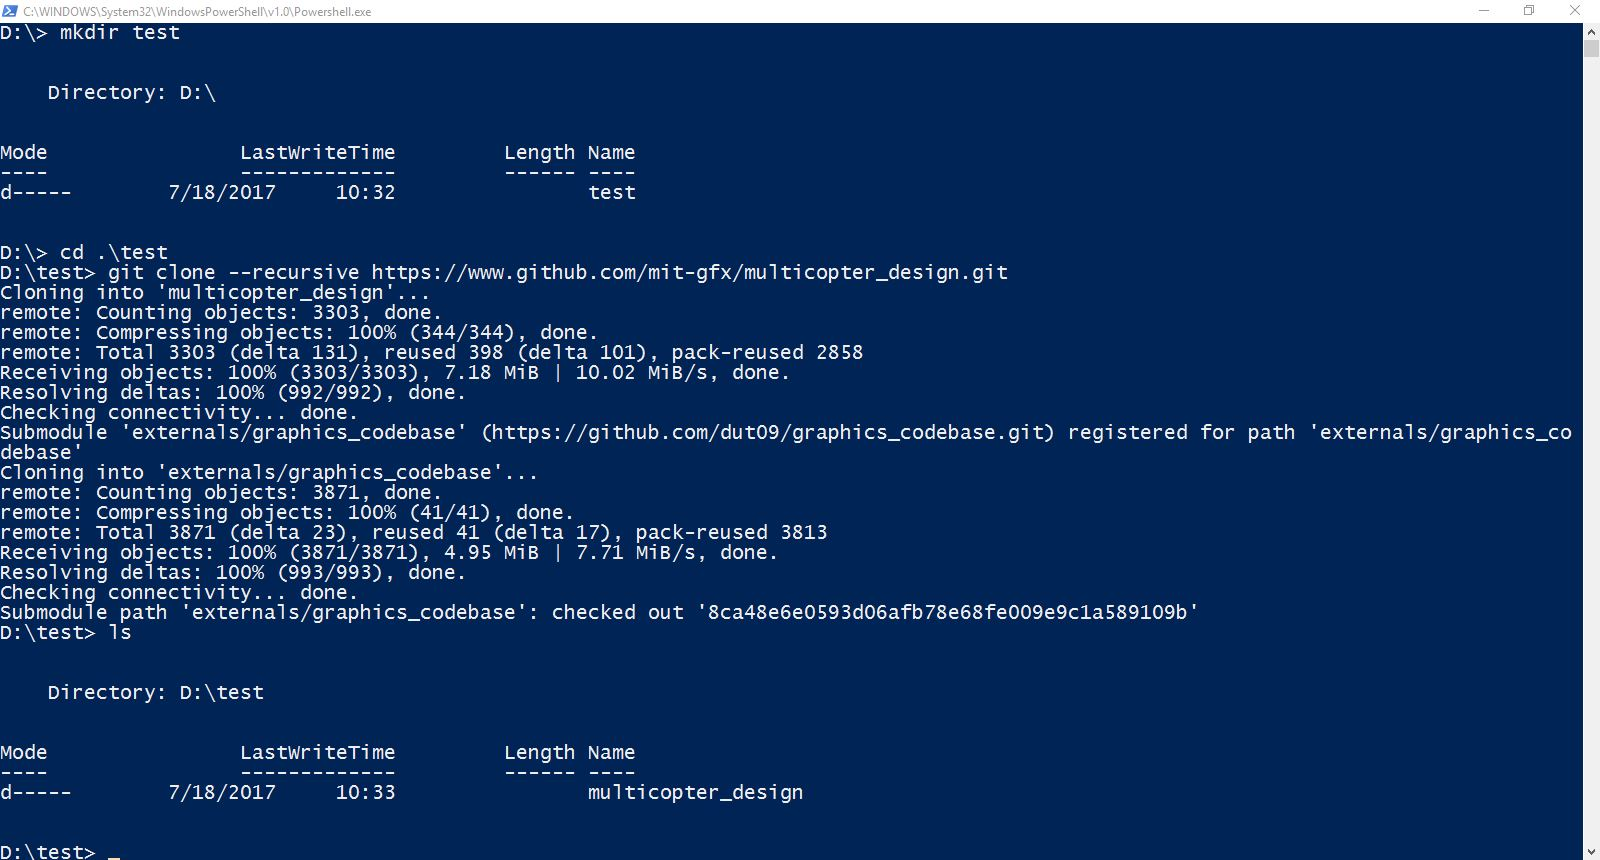
\includegraphics[width=0.75\linewidth]{windows_git_clone}
	\caption{(Windows) Cloning the project into an empty folder named \texttt{test}.}
	\label{fig:windows_git_clone}
\end{figure}

\subsubsection{Download Libraries}
Our program relies on some 3rd party libraries. Please use the provided PowerShell script to download and configure them:
\begin{verbatim}
> cd multicopter_design
> ./windows_setup.ps1
\end{verbatim}

\subsubsection{Generate the Build Solution}
\begin{figure}[!htb]
  \centering
  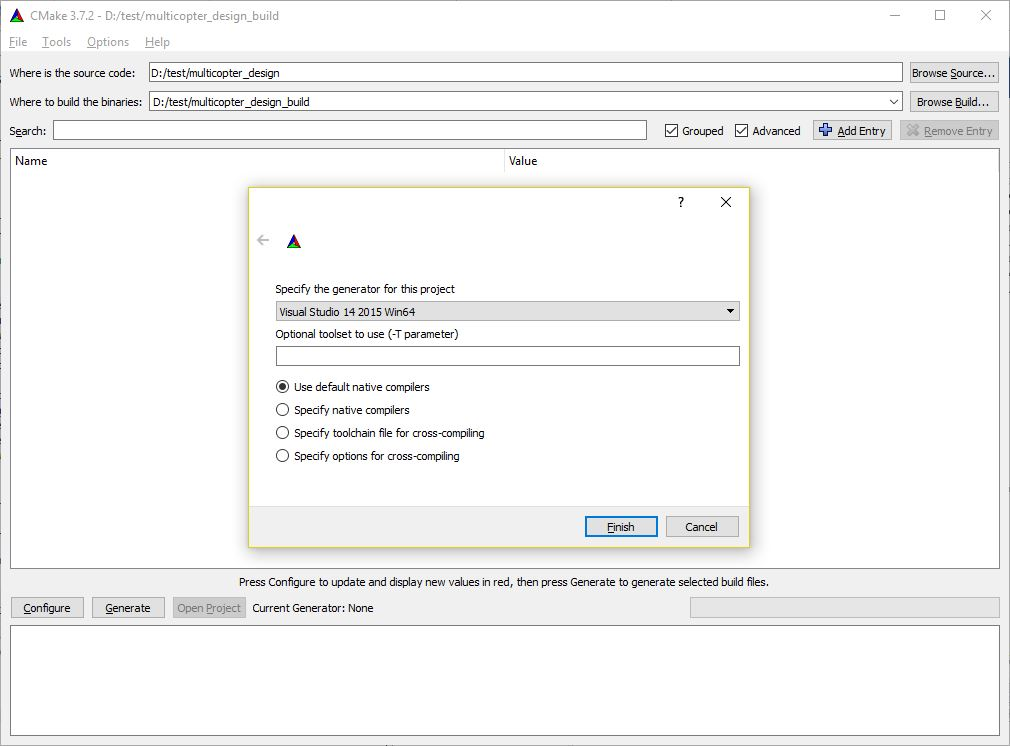
\includegraphics[width=0.75\linewidth]{windows_cmake_code_locations}
  \caption{(Windows) Using CMake to generate the build solution.}
  \label{fig:windows_cmake_code_locations}
\end{figure}
Open CMake GUI. In ``Where is the source code'', type the project location you cloned just now, which is \texttt{D:/test/multicopter\_design} in our case. For ``Where to build the binaries'', use the location you want to put the generated solution file into. Ideally it should be an empty folder out of the source. In our demo we use an empty folder located at \texttt{D:/test/multicopter\_design\_build}. Click ``Configure'', CMake will pop up a window and ask you to choose the generator. Here \texttt{Visual Studio 14 2015 Win64} is select, and you should use the C\texttt{++} IDE you have installed on your computer (Figure~\ref{fig:windows_cmake_code_locations}), click ``Finish'' when you are ready.

During the configuration step, CMake will display a few messages and finally ``Configuring done'' if no error occurs. Click ``Generate'' to create the Visual Studio solution file, which can be found in the location you specified in ``Where to build the binaries''. Click ``Open Project'' and wait for Visual Studio to open your solution.

\subsubsection{Build and Test}
After Visual Studio is open and ready, press \texttt{F7} or click ``Build'' on the menu and choose ``Build Solution''. The default configuration is built in ``Debug'' mode but you can also switch to ``Release'' for faster solution. If no error occurs, multiple executable files will be generated in the folder you used for building binaries. Now set \texttt{copter\_viewer} as the startup project and press \texttt{F5}. A window should pop up and you will see a copter with 5 rotors in the middle (Figure~\ref{fig:windows_default_ui}).
\begin{figure}[!htb]
	\centering
	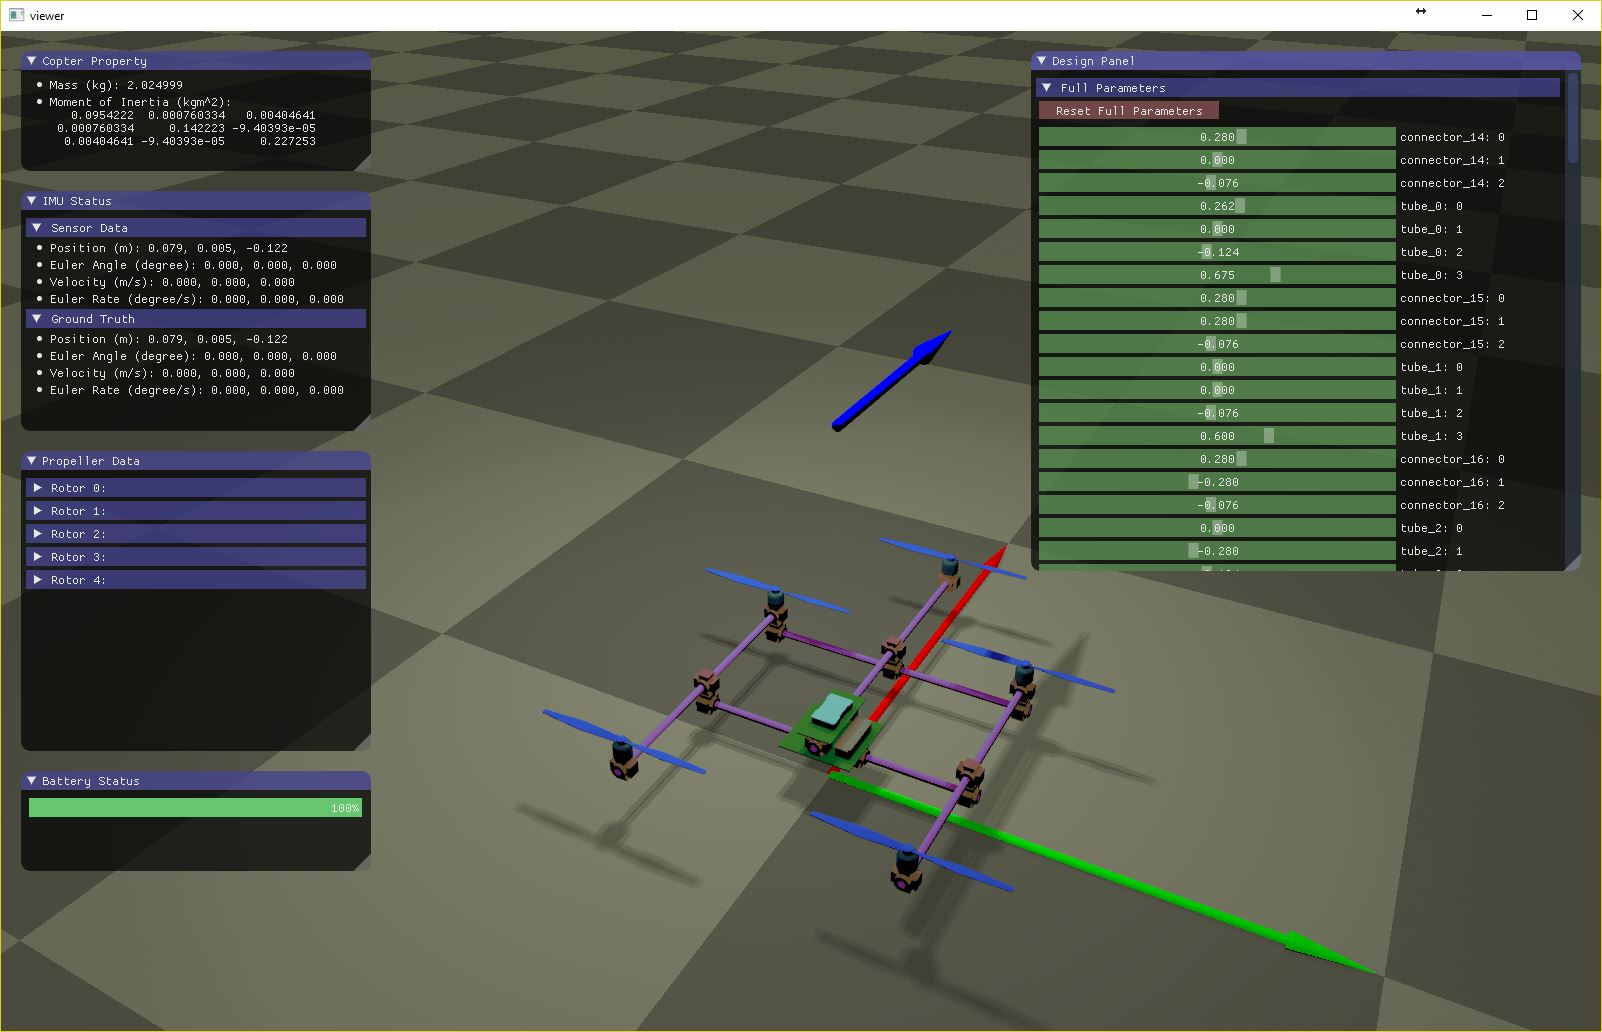
\includegraphics[width=0.75\linewidth]{windows_default_ui}
	\caption{(Windows) A screenshot of the user interface after a successful build.}
	\label{fig:windows_default_ui}
\end{figure}

\subsection{Build on Linux}
This tutorial has been tested on Ubuntu 16.04 LTS 64bit with gcc/g\texttt{++} 4.9.4.

\subsubsection{Install OpenGL libraries} Before you clone our project, make sure all the following libraries have been installed:
\begin{verbatim}
> sudo apt-get update
> sudo apt-get upgrade
> sudo apt-get install libgl1-mesa-dev mesa-common-dev xorg-dev
> sudo apt-get install libglu1-mesa libglu1-mesa-dev
\end{verbatim}
Figure~\ref{fig:ubuntu_opengl_install} is provided for your reference if you encounter any errors and are interested in knowing the exact version of these libraries we are using:
\begin{figure}[!htb]
  \centering
  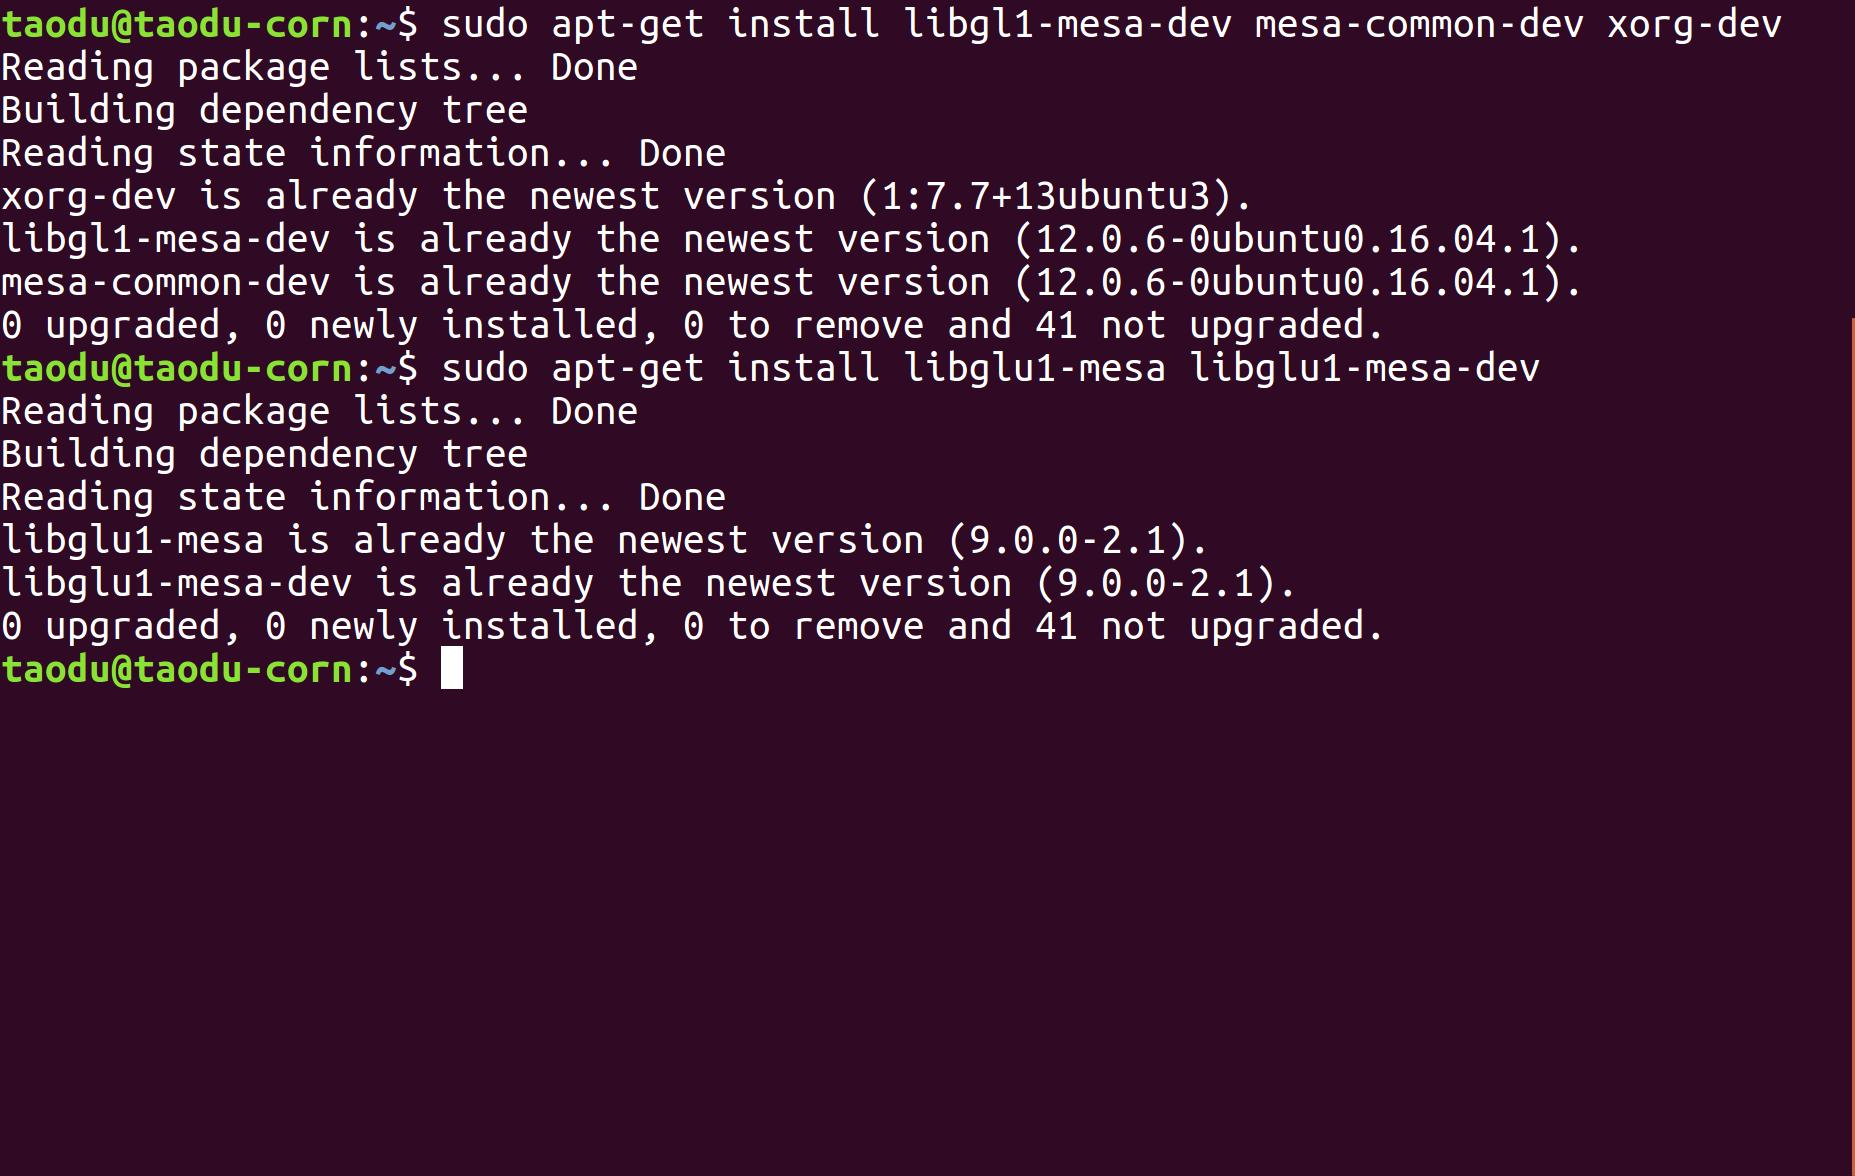
\includegraphics[width=0.75\linewidth]{ubuntu_opengl_install}
  \caption{(Ubuntu) Installing prerequisites.}
  \label{fig:ubuntu_opengl_install}
\end{figure}

\subsubsection{Get the Source Code from GitHub}
Create an empty folder, then use \texttt{git} to clone the project.
\begin{verbatim}
> mkdir test
> cd test
> git clone --recursive https://github.com/mit-gfx/multicopter_design.git
\end{verbatim}

\subsubsection{Download Libraries}
Our program relies on some 3rd party libraries. Please use the provided script to download and configure them:
\begin{verbatim}
> cd multicopter_design
> ./linux_setup.sh
> cd ../
\end{verbatim}

\subsubsection{Generate Makefile}
Next, you will need CMake to generate a Makefile for compiling the code. As before we recommend an out-of-source build. In Figure~\ref{fig:ubuntu_cmake_code_location}, we create an empty folder named \texttt{test/multicopter\_design\_build}, and a Makefile is generated inside.
\begin{verbatim}
> mkdir multicopter_design_build
> cd multicopter_design_build
> cmake ../multicopter_design
\end{verbatim}

\begin{figure}[!htb]
  \centering
  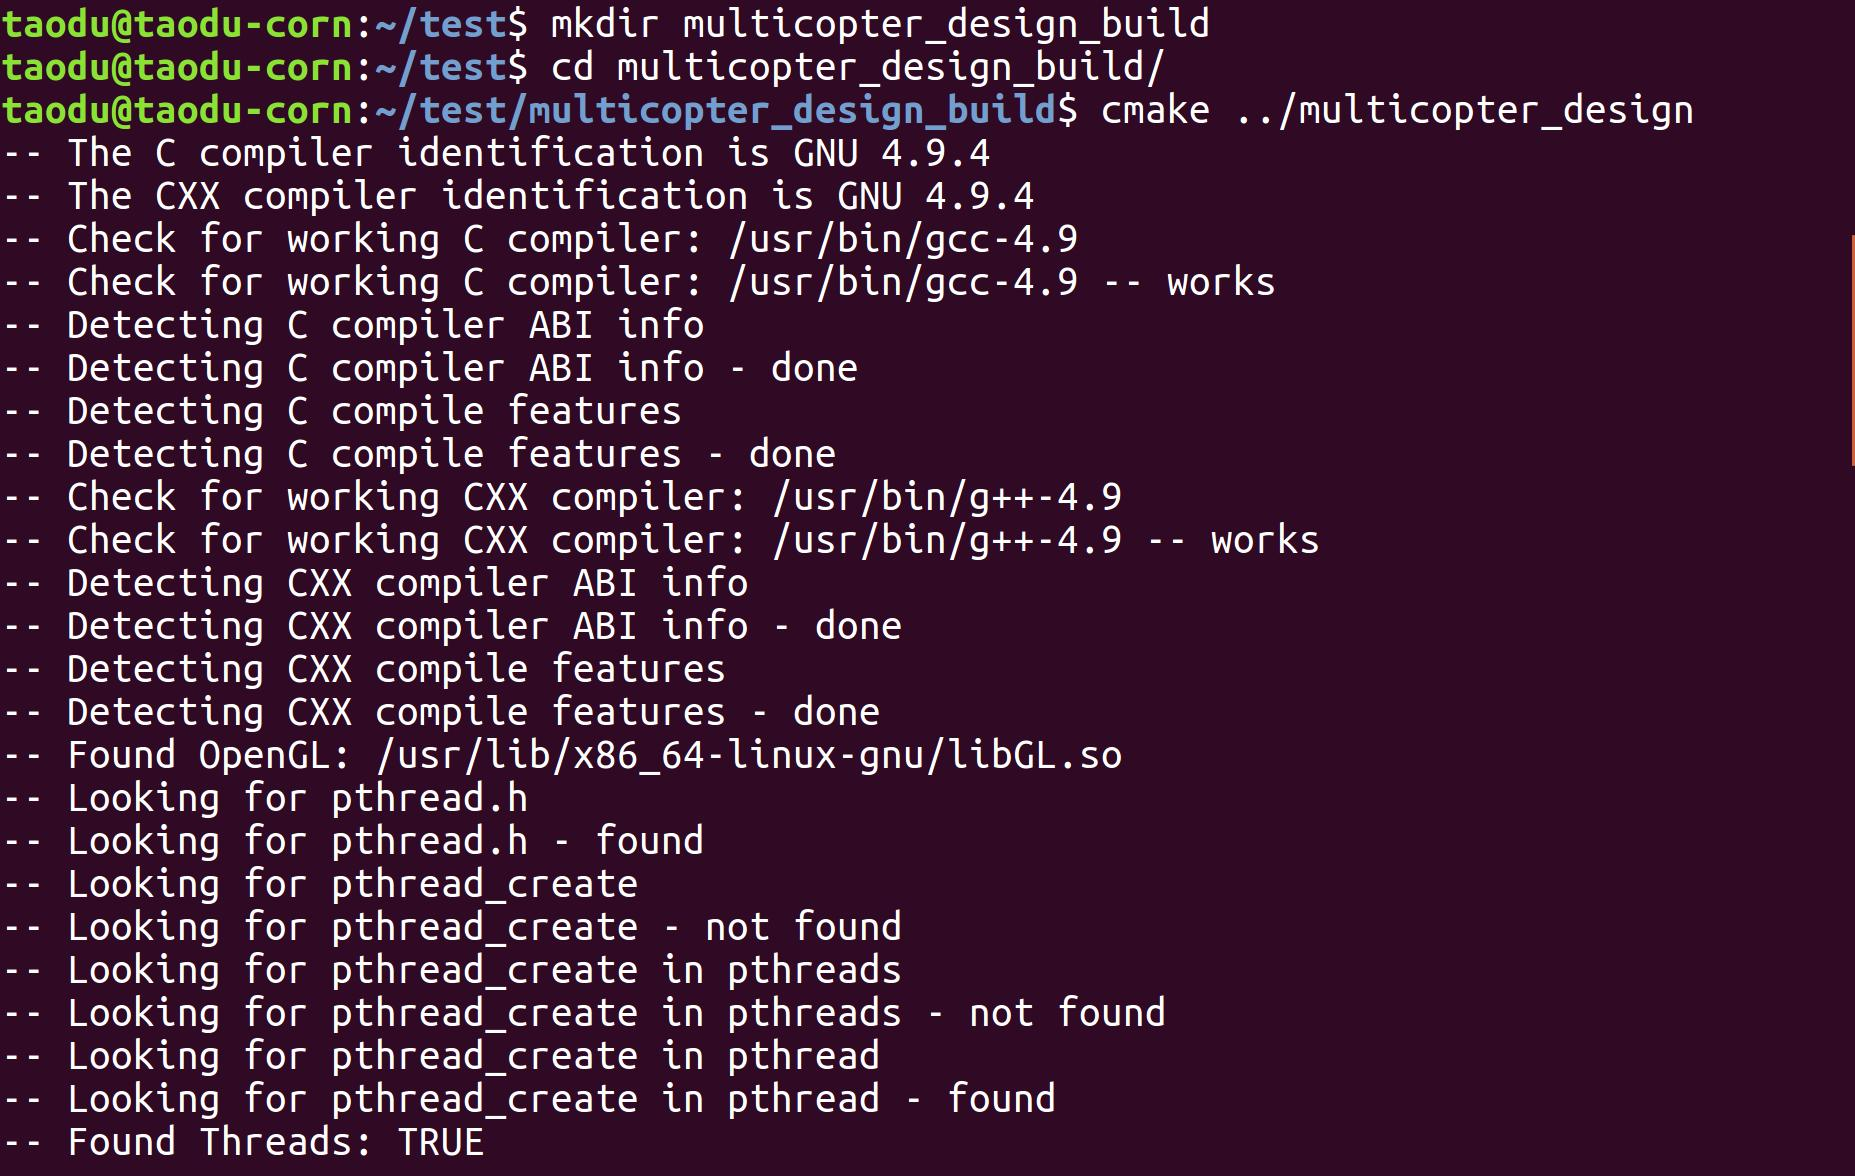
\includegraphics[width=0.75\linewidth]{ubuntu_cmake_code_location}
  \caption{(Ubuntu) Using CMake to generate a Makefile.}
  \label{fig:ubuntu_cmake_code_location}
\end{figure}

\subsubsection{Build and Test}
Once a Makefile is generated, you can call \texttt{make} to build it. If no errors occur, an executable file \texttt{copter\_viewer} will be generated. To test if the build is successful, try running \texttt{copter\_viewer} without any arguments (Figure~\ref{fig:ubuntu_run}), and a window like Figure~\ref{fig:ubuntu_default_ui} should pop up.
\begin{verbatim}
> make
> cd projects/copter_viewer/
> ./copter_viewer
\end{verbatim}

\begin{figure}[!htb]
  \centering
  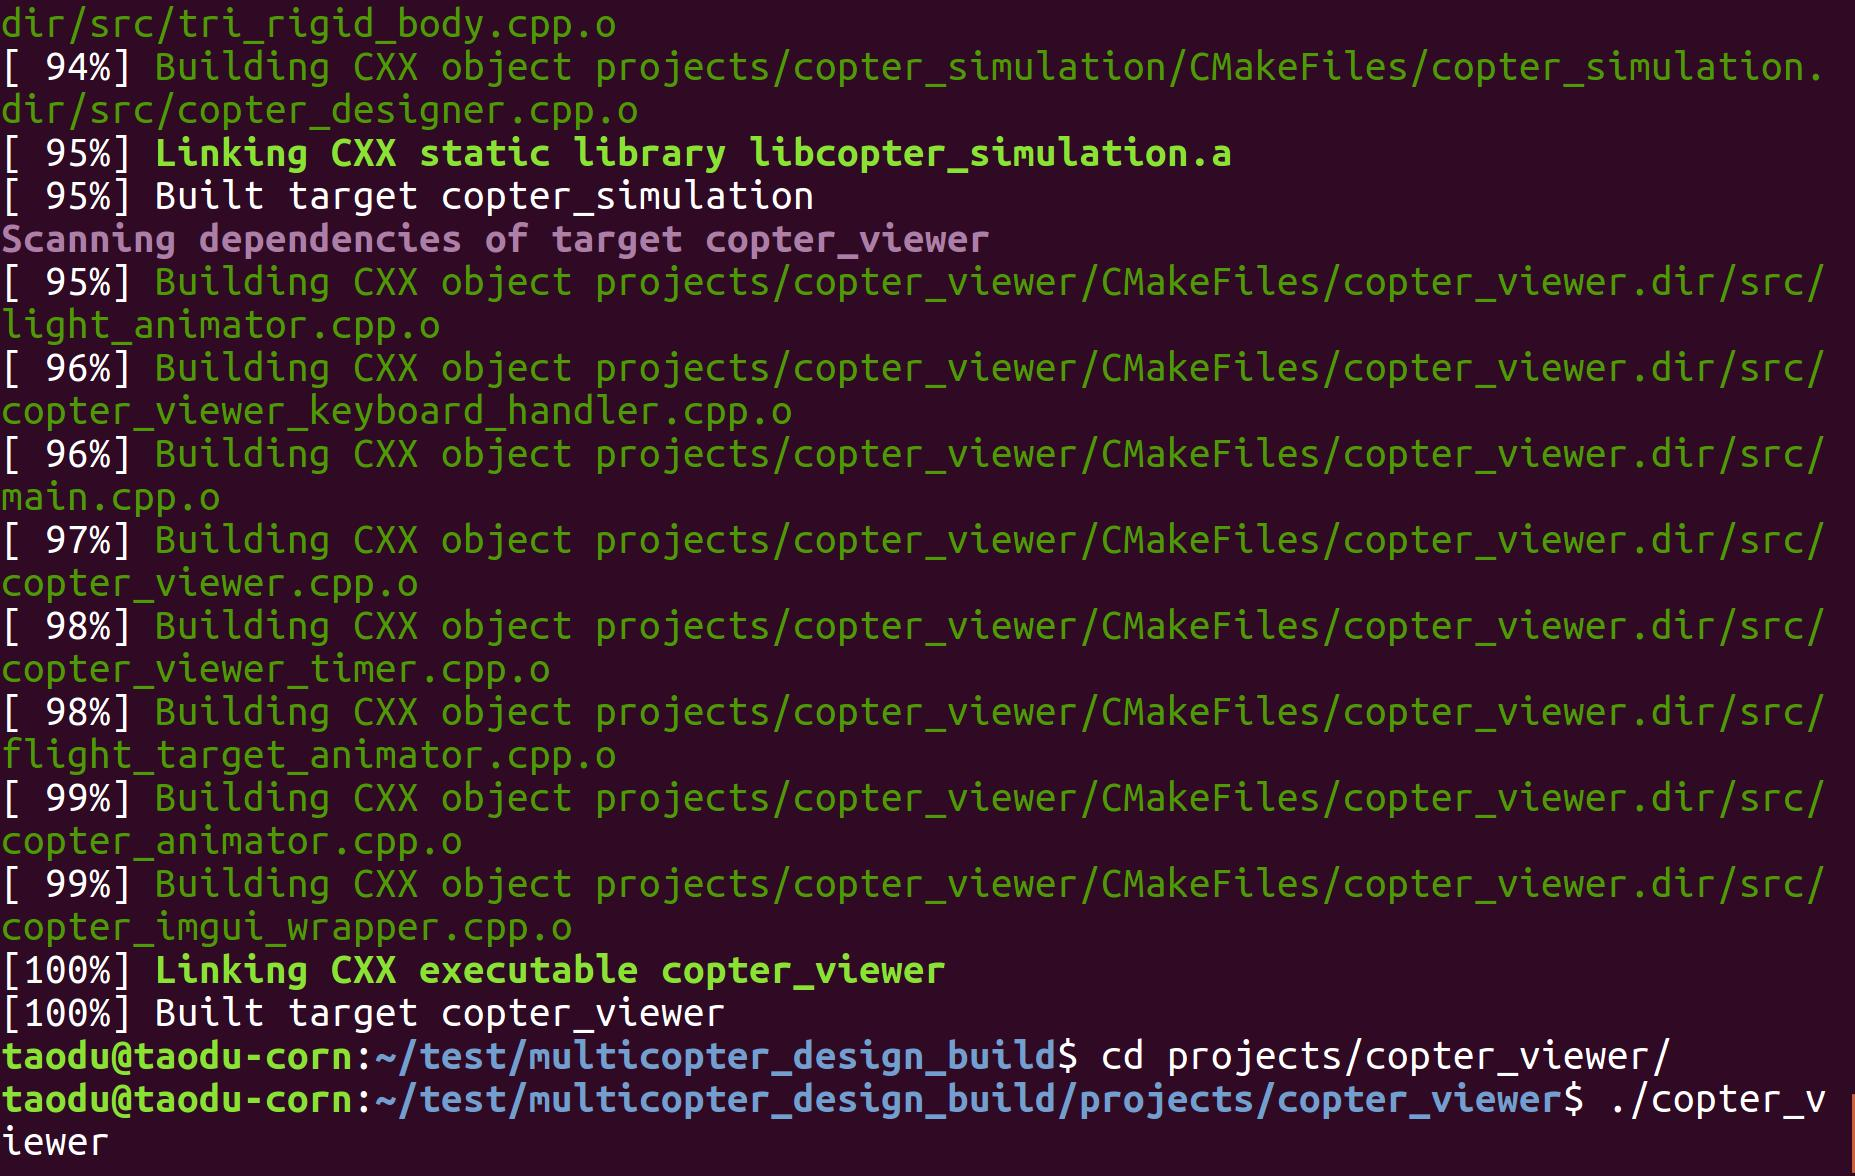
\includegraphics[width=0.75\linewidth]{ubuntu_run}
  \caption{(Ubuntu) Running \texttt{copter\_viewer} without any arguments.}
  \label{fig:ubuntu_run}
\end{figure}
\begin{figure}[!htb]
  \centering
  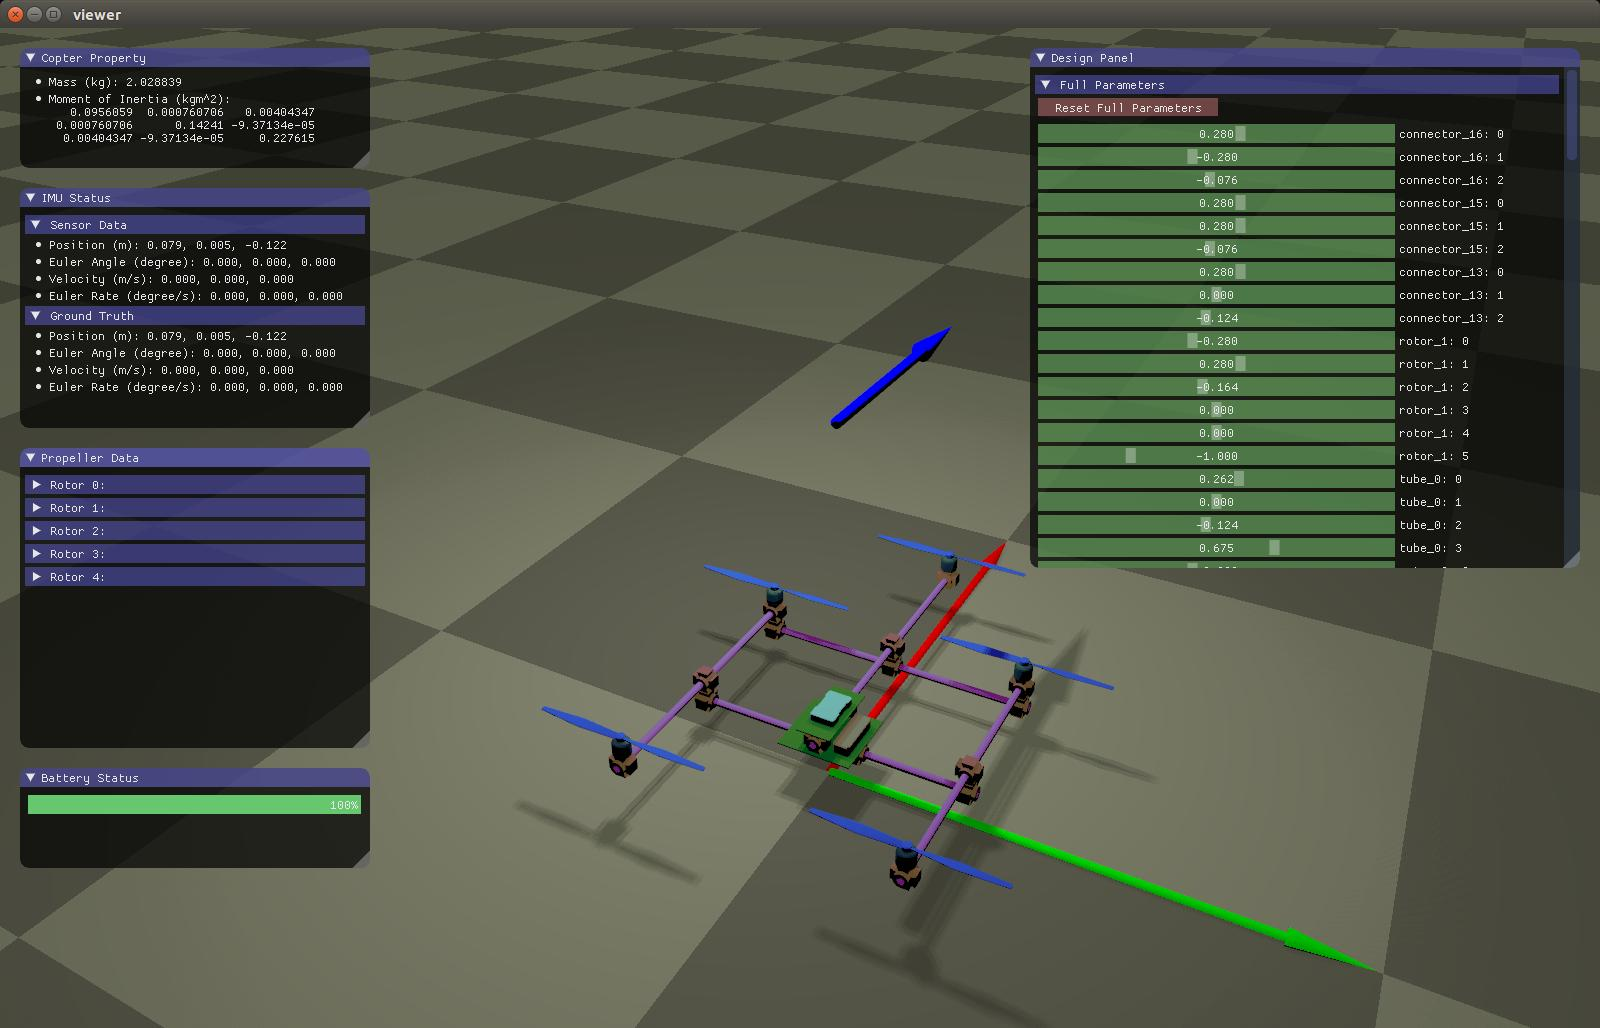
\includegraphics[width=0.75\linewidth]{ubuntu_default_ui}
  \caption{(Ubuntu) A screenshot of the user interface after we build from the source code.}
  \label{fig:ubuntu_default_ui}
\end{figure}

\subsection{Build on macOS}
The following tutorial has been tested on macOS Sierra (10.12.3) with AppleClang 8.1.0 provided in Xcode. The build steps are almost identical to those on Linux, except that no manual OpenGL installation is needed.

\begin{figure}[!htb]
  \centering
  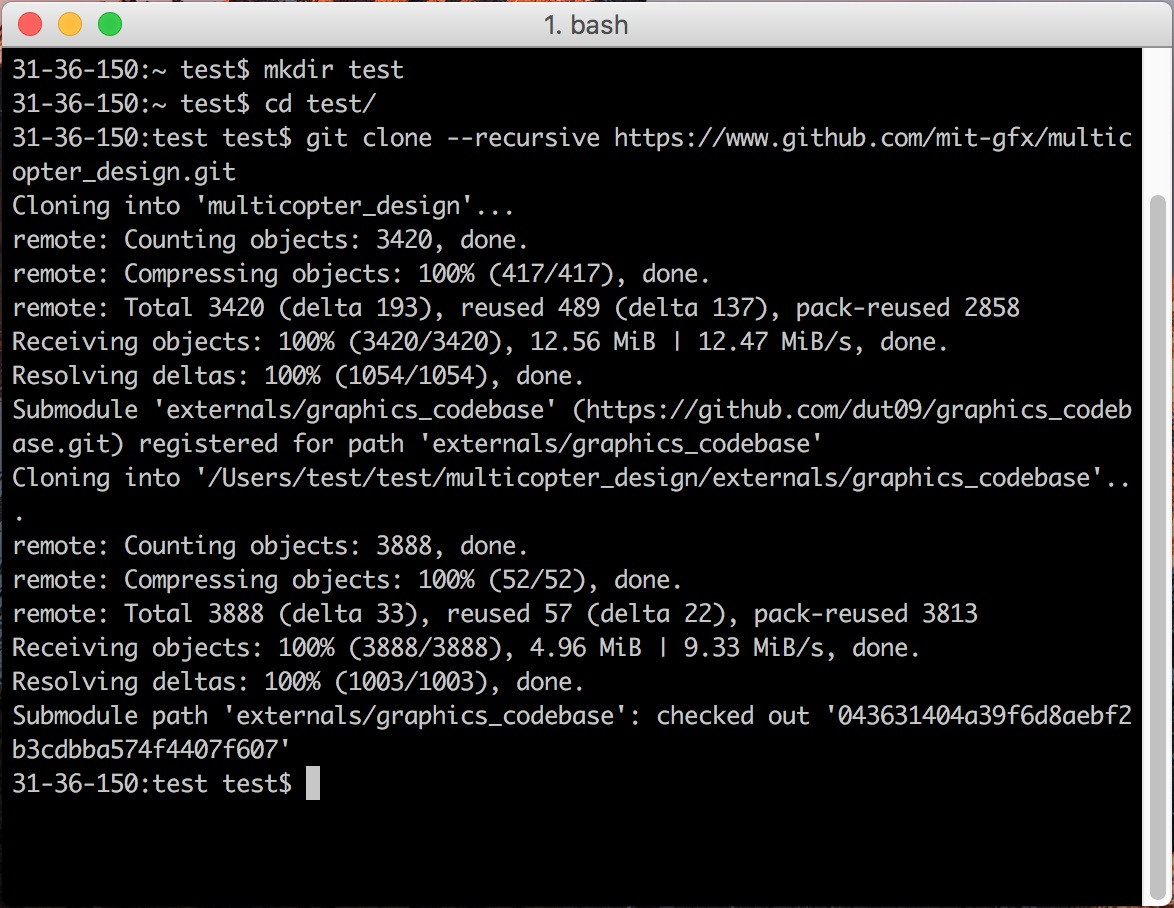
\includegraphics[width=0.75\linewidth]{macos_git_clone}
  \caption{(macOS) Cloning the project into an empty \texttt{test/} folder.}
  \label{fig:macos_git_clone}
\end{figure}
\subsubsection{Get the Source Code from GitHub}
Create an empty folder, then use \texttt{git} to clone the project. In Figure~\ref{fig:macos_git_clone} we cloned it into a newly created empty folder \texttt{test/}:
\begin{verbatim}
> mkdir test
> cd test
> git clone --recursive https://github.com/mit-gfx/multicopter_design.git
\end{verbatim}

\subsubsection{Download Libraries}
Our program relies on some 3rd party libraries. Please use the provided script to download and configure them:
\begin{verbatim}
> cd multicopter_design
> ./macos_setup.sh
> cd ../
\end{verbatim}

\subsubsection{Generate Makefile}
Next, you will need CMake to generate a Makefile for compiling the code. We recommend an out-of-source build. In Figure~\ref{fig:macos_cmake_code_location}, we create an empty folder named \texttt{test/multicopter\_design\_build}, and a Makefile is generated inside.
\begin{verbatim}
> mkdir multicopter_design_build
> cd multicopter_design_build
> cmake ../multicopter_design
\end{verbatim}

\begin{figure}[!htb]
  \centering
  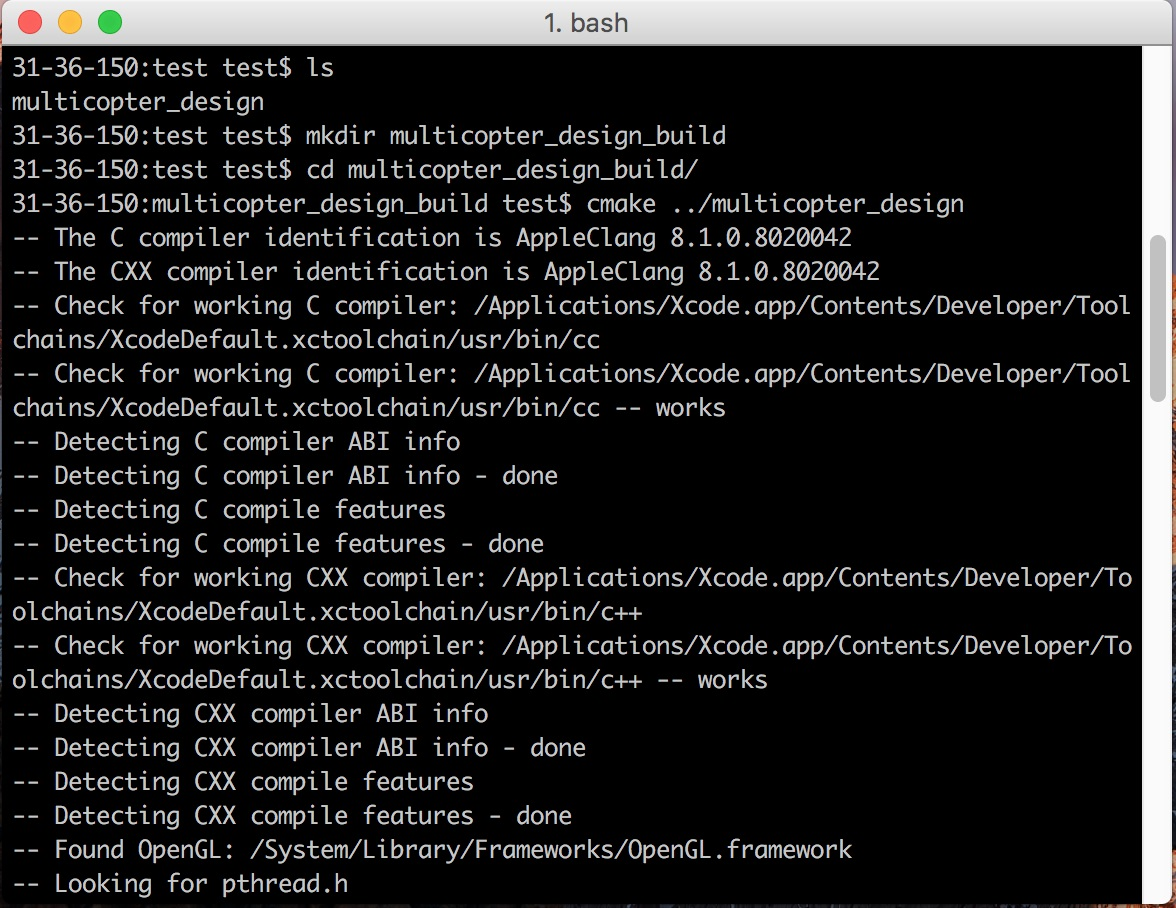
\includegraphics[width=0.75\linewidth]{macos_cmake_code_location}
  \caption{(macOS) Using CMake to generate a Makefile.}
  \label{fig:macos_cmake_code_location}
\end{figure}

\subsubsection{Build and Test}
Once a Makefile is generated, you can call \texttt{make} to build it. If no errors occur, an executable file \texttt{copter\_viewer} will be generated. To test if the build is successful, try running \texttt{copter\_viewer} without any arguments (Figure~\ref{fig:macos_run}), and a window like Figure~\ref{fig:macos_default_ui} should pop up.
\begin{verbatim}
> make
> cd projects/copter_viewer/
> ./copter_viewer
\end{verbatim}
\begin{figure}[!htb]
  \centering
  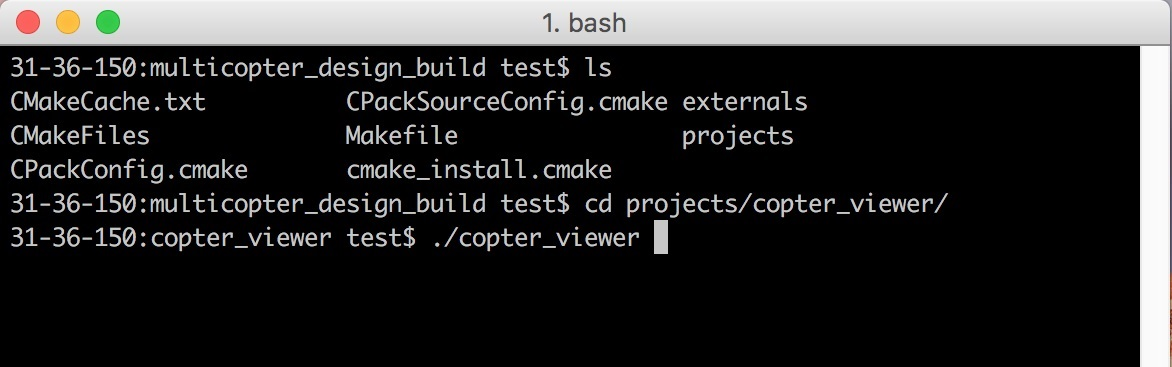
\includegraphics[width=0.75\linewidth]{macos_run}
  \caption{(macOS) Running \texttt{copter\_viewer} without any arguments.}
  \label{fig:macos_run}
\end{figure}

\begin{figure}[!htb]
  \centering
  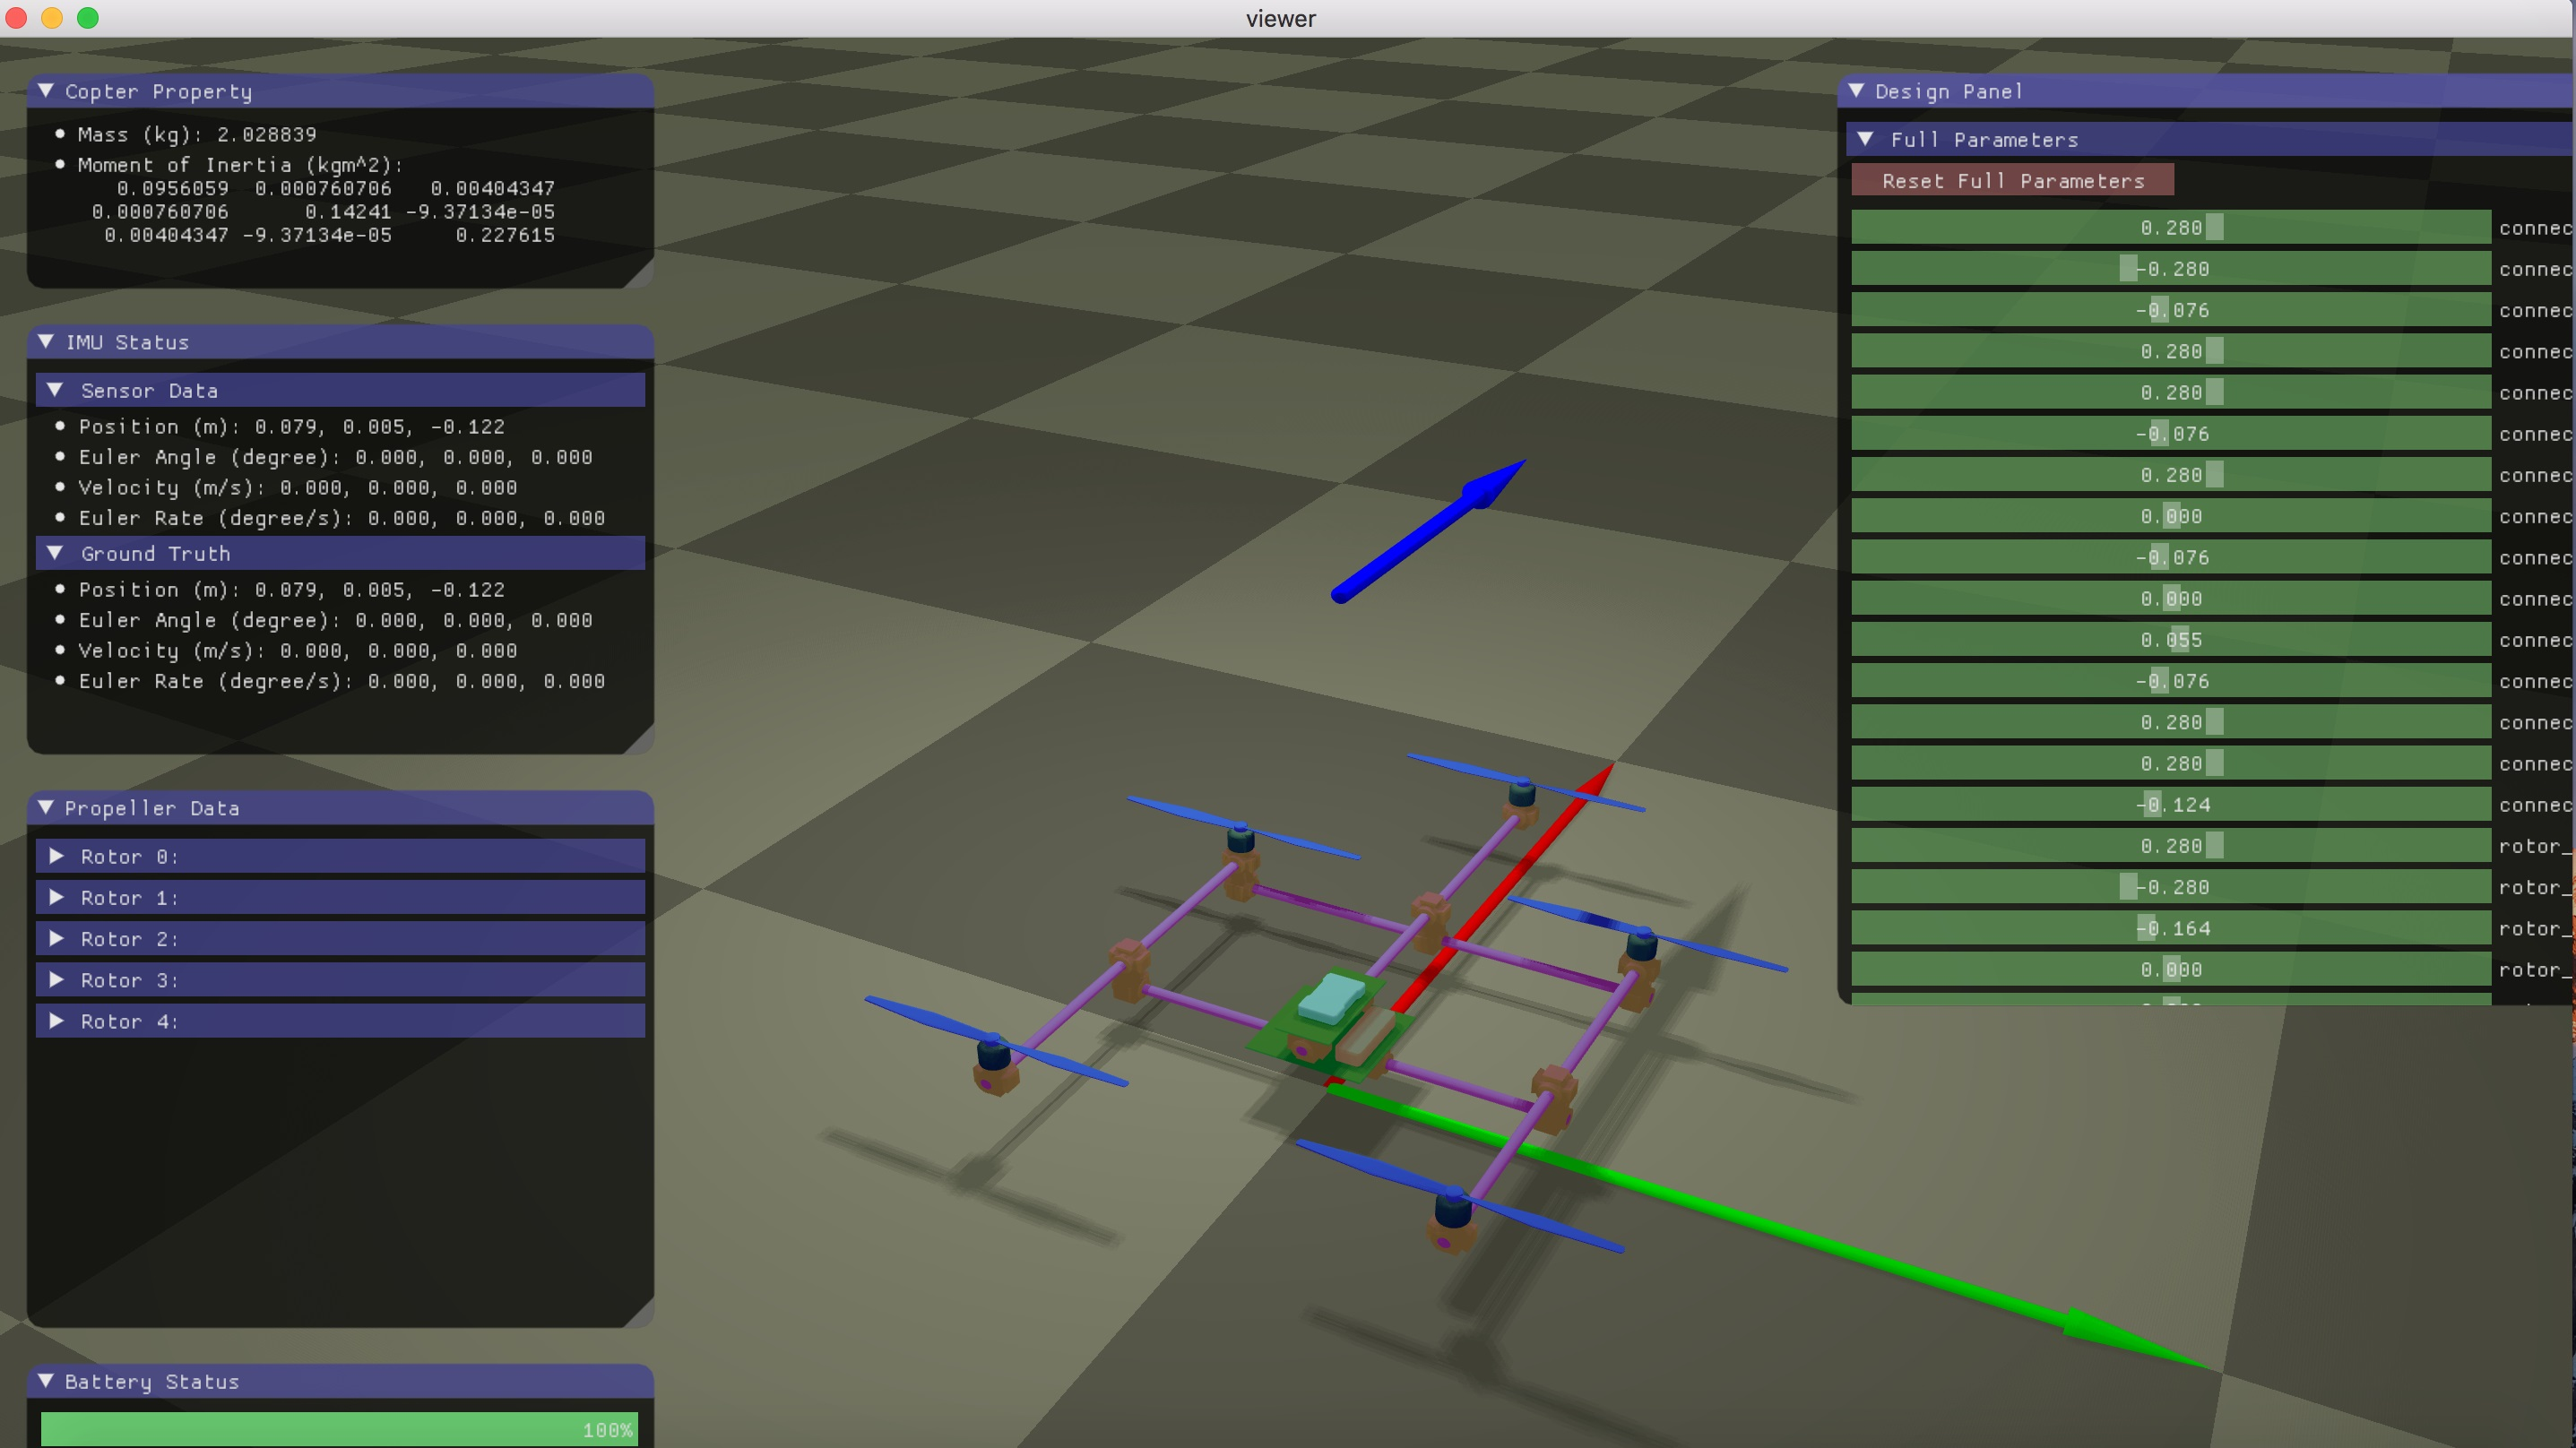
\includegraphics[width=0.75\linewidth]{macos_default_ui}
  \caption{(macOS) A screenshot of the user interface after we build from the source code.}
  \label{fig:macos_default_ui}
\end{figure}

\clearpage
\section{User Interface}\label{sec:ui}
We have briefly covered the user interface in Section~\ref{sec:intro}. Here we provide more instructions on interacting with each window. We will also explain keyboard shortcuts and mouse operations in this section.

\subsection{Copter Property Window}
This window displays mass and moment of inertia information:

\begin{itemize}
  \item \textbf{Mass} Computing mass is straightforward as it only requires summing up the mass of each part. Technically, each component is defined by a closed surface mesh and a density value. We will assume this mesh is solid and use the divergence theorem to analytically compute its mass. 

  \item \textbf{Moment of Inertia} The moment of inertia is a $3\times3$ symmetric positive semidefinite matrix, defined on a local frame $\mathcal{F}$ rigidly attached to the copter. $\mathcal{F}$ is computed and fixed once an initial design is loaded. The origin of $\mathcal{F}$ is the center of mass and its three axes are parallel to the world frame axes. Recall that the world frame we use is north-east-down, where $x$, $y$ and $z$ point to the north (red), east (green) and down (not shown in the window as it is below the ground) direction.
\end{itemize}

The moment of inertia determines the torque need to rotate the copter. It is generally recommended that you place your initial design in a way that its heading is along the $x$ axis with zero roll angle. In this way the diagonal elements in the matrix reveal the resistance of the copter to rolling, pitching, and yawing respectively.

\subsection{IMU Status Window}
This window shows the reading from a virtual sensor attached to the copter, and the ground truth status. Both consist of the following information:

\begin{itemize}
  \item \textbf{Position} These three numbers show where the center of mass is located in the world frame. As $z$ axis points down to the ground, positive altitude corresponds to a negative $z$ value.
  
  \item \textbf{Euler Angle} These are the roll, pitch and yaw angles. Initially the body axes are parallel to world axes. We first rotate it around $z$ by yaw, then rotate along the new $y$ axis of the body frame by pitch, then finally rotate around the new $x$ axis of the body frame by roll.

  \item \textbf{Velocity} The time derivative of position.

  \item \textbf{Euler Rate} The time derivative of Euler angles.
\end{itemize}

\subsection{Propeller Data Window}
This window contains information about rotors, with one sub-window for each. The rotors are ordered by their occurrence in the file. Each sub-window contains:

\begin{itemize}
  \item \textbf{Position} This shows where the motor is located in the \textbf{body} frame. Their values get updated during the design process and fixed in simulation.

  \item \textbf{Direction} This unit vector shows where this motor points to in the \textbf{body} frame. Typically it is close to $(0,0,-1)$.

  \item \textbf{Spinning} A string shown here indicates whether the propeller spins clockwisely (CW) or counter-clockwisely (CCW), defined in a view where the motor is pointing towards you.

  \item \textbf{Speed} This shows the rotation speed of the propeller, in RPM (round per minute).

  \item \textbf{Thrust} This is the magnitude of the thrust generated by the propeller.
\end{itemize}
Both speed and thrust are calculated from fitting measurement data provided in the file. Thrust is also clamped between $0$ and the measured maximum.

\subsection{Battery Status Window}
This progress bar works as an indicator of the battery life. During a flight we collect the thrust of each rotor, and based on the measurement data provided in the file, we estimate the current sent to each rotor. Dividing the remaining capacity by the current gives a rough estimation of time left before the battery becomes completely drained. The progress bar will turn yellow when it is $60\%$, and become red when below $20\%$.

\subsection{Design Panel Window}
This is the main window people will be working on when designing the copter. It consists of a sub-window that allows you to directly change full parameters, another to manipulate equivalent reduced parameters, and a simulation panel.

\subsubsection{Full Parameters}
As we will see in Section~\ref{sec:file}, parts like tubes, connectors and motors are parametrized by their geometric properties. This window displays all parameters labeled by their names, with an extension of indices. Although you are allowed to slide each single value, note that these parameters are constrained by the way you build the copter, so changing one parameter may affect the others as well.

Technically, let $\mathbf{x}$ be a vector of all parameters listed in the ``Full Parameter'' window. We build all constraints as linear functions of $\mathbf{x}$, which are compactly represented by $\mathbf{Ax}=\mathbf{b}$ and $\mathbf{Cx}\leq\mathbf{d}$. When you slide a single parameter in the window, we store all parameter values currently shown in the window into a vector $\mathbf{x}_0$, and the new $\mathbf{x}$ is determined by solving the optimization problem below:
\begin{equation}
\begin{aligned}
\min_{\mathbf{x}}&\quad \|\mathbf{x} - \mathbf{x}_0\|\\
s.t.&\quad \mathbf{Ax}=\mathbf{b}\\
&\quad \mathbf{Cx}\leq\mathbf{d}
\end{aligned}
\end{equation}
In other words, we find in the feasible set the closest solution to the parameter values indicated by users from the window.

\subsubsection{Reduced Parameters}
It is common that tens or hundreds of parameters are introduced in a design while most of them are limited by equality constraints. In this case using reduced parameters can significantly reduce the design space. Mathematically, the solution of $\mathbf{Ax}=\mathbf{b}$ can be fully characterized by vectors in its null space. Let $\mathbf{Ax}_0=\mathbf{b}$, and write $\mathbf{x}=\mathbf{x}_0+\mathbf{Ey}$ where $\mathbf{E}$ spans the null space of $\mathbf{A}$. Now the equality constraints are removed and we can focus on a much lower dimensional vector $\mathbf{y}$.

The reduced parametric representation brings its own drawbacks though. Perhaps the biggest issue here is that $\mathbf{y}$ does not have a straightforward physical meaning any more. Each element does not correspond to a single component, but might affect the global design in an unintuitive way.

Unlike the full parameters, it is easier to update the reduced parameters when they get updated in the window. Let $\mathbf{Fy}\leq{g}$ be the only inequality constraints on $\mathbf{y}$. When one $y_i$ is updated, we fix other $y_i$s and calculate the feasible range of $y_i$ and reflect it in the window. If some $y_i$ freezes on the boundary of $\mathbf{Fy}\leq\mathbf{g}$, its background then becomes red to imply this $y_i$ is not changeable.

\subsubsection{Simulation}
This window contains a button to trigger the simulation process. Your design is then set to track the position and heading of the blue arrow in the scene, which can be changed by keyboard shortcuts discussed below. All design parameters are frozen during flight unless you press the button again and switch back to the design process.

Behind this simulation button we execute a $30$Hz loop to control the flight. Within each iteration we do the following things in order:
\begin{itemize}
  \item Collect the sensor data and target information.

  \item Execute the control policy based on them.

  \item Send control signals to each rotor.

  \item Use thrust and torque from each rotor to update the motion.
\end{itemize}
Note that depending on your graphics card the actual FPS (frame per second) may be above or below 30. So the time flow you feel in the window is not exactly the actual motion you expect to see in your real copter.

\subsection{Keyboard Shortcuts}
The following keys are used as shortcuts. Most are activated only in simulation.
\begin{itemize}
  \item \textbf{Left/Right/Up/Down Arrow} This four keys control the horizontal position of the target (blue arrow in the window). The default controller will try to drag the copter to track the blue arrow as close as possible.

  \item \textbf{`w' and `s'} These two keys adjust the vertical location of the blue arrow, which in turn controls the altitude of the copter.

  \item \textbf{`a' and `d'} These keys rotate the blue arrow on the horizontal plane, which changes the desired heading of the copter in simulation.

  \item \textbf{`p'} When pressing `p' you can pause/resume the simulation.
\end{itemize}

\subsection{Mouse Operations}
Mouse gestures are used to control the camera view. Specifically, the following operations are supported:
\begin{itemize}
  \item \textbf{Zooming in/out} By scrolling the mouse wheel you can zoom the camera to get closer/farther to the scene.

  \item \textbf{Rotation} You can press the mouse wheel and drag to rotate the camera.

  \item \textbf{Panning} Press shift and the mouse wheel and drag your mouse at the same time to change the camera location.
\end{itemize}

\clearpage
\section{File Format}\label{sec:file}
We use XML files to define the copter used in our design and simulation tool. A list of sample files are provided in the folder \texttt{resources/copter/} for your reference. To load an XML file, simply use its name as the first argument when you run \texttt{copter\_viewer}. For example:
\begin{verbatim}
> ./copter_viewer y6copter.xml
\end{verbatim}
will load a Y6 hexacopter defined in \texttt{y6copter.xml} (Figure~\ref{fig:y6_ui}). If no XML file is given, then \texttt{pentacopter.xml} is used by default.
\begin{figure}[htb]
	\centering
	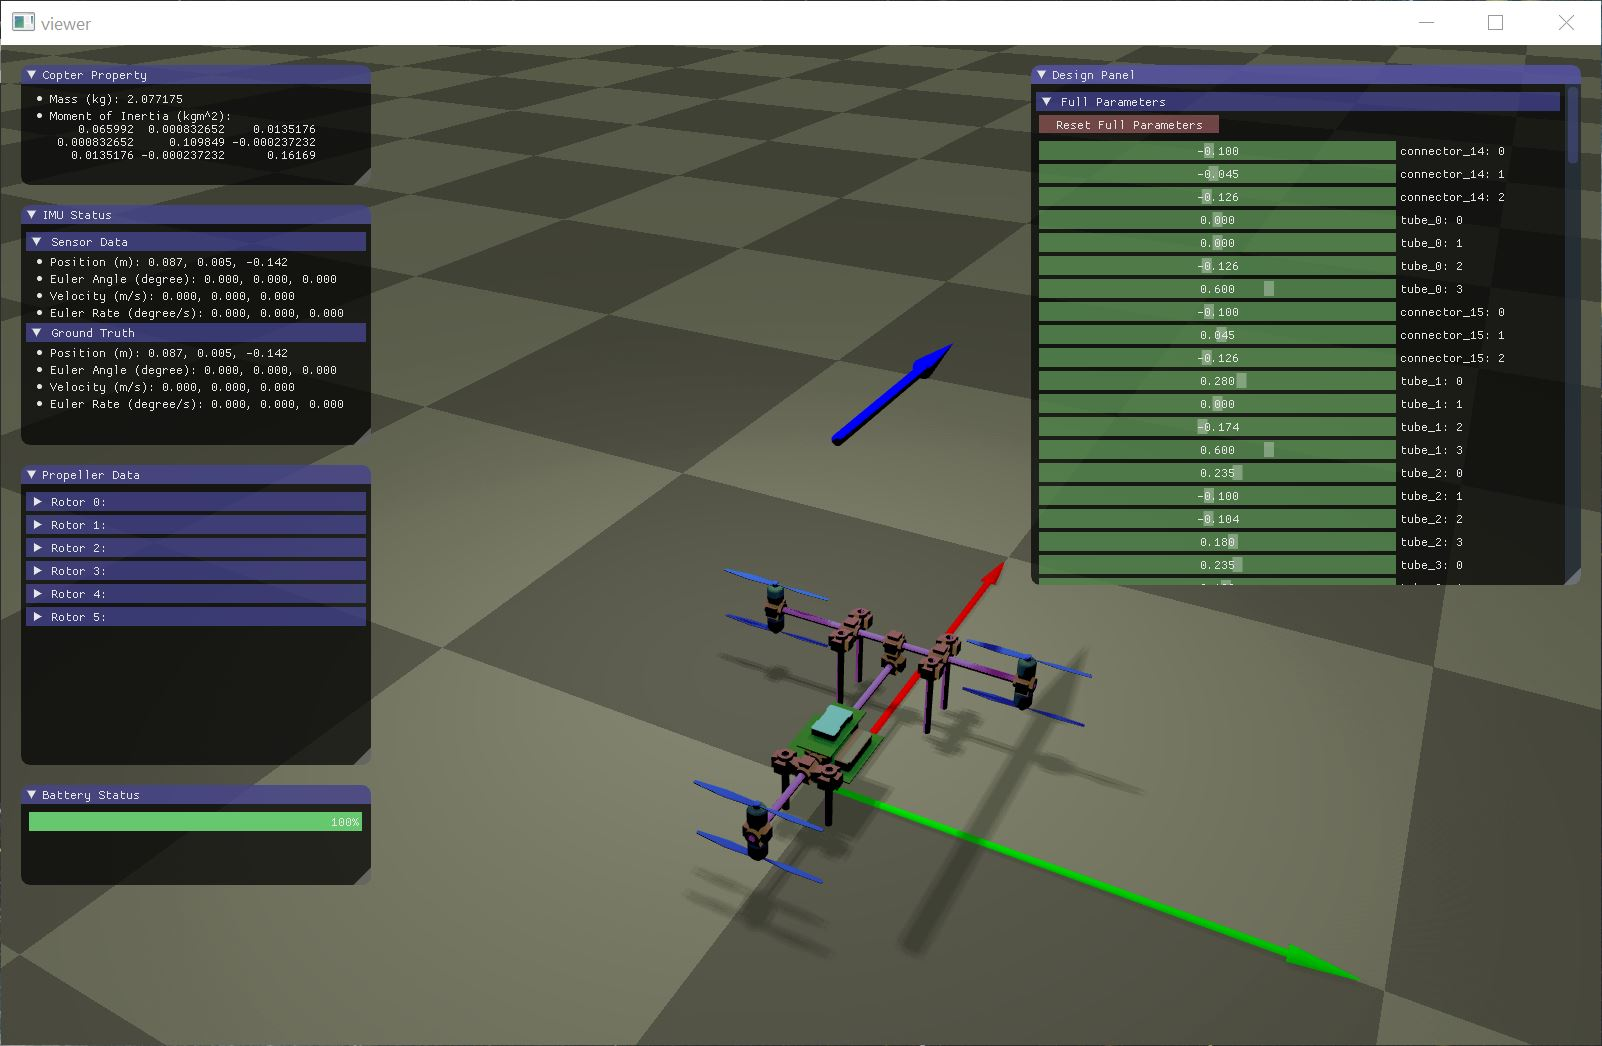
\includegraphics[width=1.0\linewidth]{y6_ui}
	\caption{Loading a Y6 hexacopter from the given XML file \texttt{y6copter.xml}.}
	\label{fig:y6_ui}
\end{figure}

The XML file itself its pretty straightforward: once you learn the rules, you are free to create your own XML files and use the software to design and simulate them. For simplicity, below we will walk you through \texttt{quadcopter.xml} so that you can get an idea of how to write your own copter file.

\subsection{Basic Structure}
The XML file starts with a line defining the version:
\begin{verbatim}
<?xml version="1.0" ?>
\end{verbatim}

The whole copter is then wrapped by a pair of tags \texttt{<copter>} and \texttt{</copter>}. You should put all your components inside these opening and closing tags. To define a complete copter, you will have to provide definitions for the following components: plates, a battery, an electronic device, tubes, connectors, propellers, and motors. All meshes used here must be watertight, otherwise we won't be able to estimate their moment of inertia.

\subsection{3D Transforms}
Many of the components are defined in their own frames in the mesh file. To place them correctly you need to apply a series of transforms. In the XML file you can specify it by using \texttt{translate} and \texttt{rotate} tags. Scaling is in general not supported except for plates and tubes.

To apply a translation, use the following tag:
\begin{verbatim}
<translate xyz="0 1 2"/>
\end{verbatim}
Applying it will move the mesh by $(0,1,2)$.

Rotation is defined by Euler angles $(\phi,\theta,\psi)$, which are also known as roll, pitch and yaw. We first rotate the mesh along its own $z$ axis by $\psi$, then around its own (new) $y$ axis by $\theta$, finally along its (new) $x$ axis by $\phi$. The angles are in degrees and its sign is defined by the right-hand rule.
\begin{verbatim}
<rotate xyz="0 0 90"/>
\end{verbatim}
In this example, we rotate the mesh by 90 degrees around its own $z$ axis.

You can apply a series of translation/rotation to a single mesh. For example, if you want to translate it first by $(0, 1, 2)$, then rotate it by $(45, 0, 90)$, then translate it by $(3, 4, 5)$:
\begin{verbatim}
<translate xyz="0 1 2"/>
<rotate rpy="45 0 90"/>
<translate xyz="3 4 5"/>
\end{verbatim}

We will see many 3D transform examples shortly.

Finally, the world frame in which we define the copter is NED (north east down), which means \textbf{negative} $z$ is the \textbf{up} direction. To avoid penetrating the ground, we usually lift our copter a little in the definition.

\subsection{Add Plates}
To define a plate, you will need to first create the tag \texttt{<plate>} and \texttt{</plate>} with two attributes: \texttt{file} specifies the mesh file, and \texttt{density} defines its density:
\begin{verbatim}
<plate file="plate.obj" density="1180.0">
  ...
</plate>
\end{verbatim}
In our code, we look for a file named \texttt{plate.obj} in the folder \texttt{resources/mesh}, which we have provided along with the source code. This mesh is a 1m$\times$1m$\times$0.0024m axis-aligned cuboid centered at the origin, and the unit of the density value is kg$/$m$^3$.

Between \texttt{<plate>} and \texttt{</plate>} you can create multiple plates by using \texttt{<instance>} tag, one for each plate. An \texttt{<instance>} tag needs you to specify the size of your plate along $x$ and $y$ direction first, then specify the location and orientation of the plate by applying translation or rotation.
\begin{verbatim}
<instance size="0.15 0.15">
  <translate xyz="0 0 -0.1"/>
</instance>
\end{verbatim}
Here we define our first plate: it is a $0.15$m$\times0.15$m$\times0.0024$m cuboid, and it is lifted by $0.1$ meters. The second plate has a smaller size ($0.15$m$\times0.07$m), and it is lifted by $0.148$ meters, leaving a $0.048-0.0024=0.0456$ meters gap between them. This is exactly the size of one connector, which we will cover shortly:
\begin{verbatim}
<instance size="0.15 0.07">
  <translate xyz="0 0 -0.1"/>
  <!-- 0.0024m is the thickness of the plate. -->
  <translate xyz="0 0 -0.0024"/>
  <!-- 0.0456m is the size of the connector. -->
  <translate xyz="0 0 -0.0456"/>
  <!-- Instead of copying and pasting the three translations here, we will
       use -0.148 = -0.1 - 0.0024 - 0.0456 below. -->
</instance>
\end{verbatim}

Plates do not have any free parameters in the design. Once they are defined in the XML, they cannot be changed any more.

\subsection{Add Batteries}
Batteries are defined by \texttt{<battery>}, which requires a file name, a density value (in kg$/$m$^3$) and its capacity (in mAh). The density is estimated by using the mass and size from the manufacturer. Currently only one battery is allowed:
\begin{verbatim}
<battery file="battery.obj" density="2857.1" capacity="2200">
  <rotate rpy="0 0 90"/>
  <translate xyz="0 0 -0.1"/>
</battery>
\end{verbatim}
As before, you can find \texttt{battery.obj} in \texttt{resources/mesh}. In that file, we intentionally set the mesh in a position such that it is attached to \texttt{plate.obj} seamlessly. So by lifting the battery to $0.1$ meters above the ground, it is now attached to the lower plate we defined earlier.

Like plates, batteries are not parametrized in the design.

\subsection{Add Electronic Devices}
An electronic device is defined by \texttt{<electronics>} and \texttt{</electronics>}. It is only used for visualization. We also assume there is only one device needed in a copter:
\begin{verbatim}
<electronics file="electronics.obj" density="601.6">
  <!-- The electronic device is placed on top of the upper plate. -->
  <translate xyz="0 0 -0.148"/>
  <!-- Lift by 0.01 more because the mesh itself has thickness. -->
  <translate xyz="0 0 -0.01"/>
</electronics>
\end{verbatim}
\texttt{electronics.obj} defines a mesh bounded by a $0.0816$m$\times0.05$m$\times0.0154$m box and centered at the origin.

Like plates and batteries, the location and size of an electronic device are fixed once it is defined in the XML file.

\subsection{Add Tubes}
Tubes are defined between \texttt{<tube>} and \texttt{</tube>}. Each tube needs you to specify the length and location:
\begin{verbatim}
<tube file="tube.obj" density="1638.9">
  <instance length="0.5">
    <translate xyz="0 0 -0.1"/>
    <!-- 0.0012 is half of the thickness of a plate. -->
    <translate xyz="0 0 0.0012"/>
    <!-- 0.0228 is half of the size of a connector. -->
    <translate xyz="0 0 0.0228"/>
  </instance>
  <instance length="0.5">
    <rotate rpy="0 0 90"/>
    <translate xyz="0 0 -0.1"/>
    <!-- 0.0012 is half of the thickness of a plate. -->
    <translate xyz="0 0 -0.0012"/>
    <!-- 0.0228 is half of the size of a connector. -->
    <translate xyz="0 0 -0.0228"/>
  </instance>
  <!-- For simplicity we will use -0.076 and -0.124 below. -->
</tube>
\end{verbatim}
The default \texttt{tube.obj} is a 1-meter-long tube centered at the origin, and pointing along the $x$ axis. Here two 0.5-meter-long tubes are defined, one below the lower plate ($z=-0.1$) by $0.24$m and the other rotated by 90 degrees and then between two plates ($z=-0.1$ and $z=-0.148$).

A tube is parametrized by its center of mass (3 degrees of freedom) and length (1 degree of freedom), but its direction is fixed in the design.

\subsection{Add Connectors}
Connectors are defined between \texttt{<round\_connector} and \texttt{</round\_connector>}:
\begin{verbatim}
<round_connector file="connector.obj" density="1170.0">
  <instance>
    ...
  </instance>
  ...
</round_connector>
\end{verbatim}
The default mesh file \texttt{connector.obj} defines a mesh that is centered at the origin, with a bounding box of size $0.04$m$\times0.0456$m$\times0.0456$m. Without any transform, a connector will be placed at the center of \texttt{tube.obj} and allow the default tube to pass through. It is crucial to place them in the right position, otherwise our algorithm won't be able to parse their connection and constraints correctly.

As an example, consider the first connector we defined after \texttt{<round\_connector>}:
\begin{verbatim}
<instance>
  <rotate rpy="0 0 90"/>
  <translate xyz="0 0 -0.124"/>
</instance>
\end{verbatim}
So we first rotate the connector along $z$ axis by $90$ degrees, then place it at $(0,0,-0.124)$. Recall that our second tube is placed at $(0,0,-0.124)$ and points to the $y$ direction. In this way, the tube passes through the connector precisely. The value $-0.124$ comes from the half size of the connector ($0.0228$), the half of the thickness of the plate $(0.0012)$, and the offset of the lower plate ($-0.1$), which sums up to $-0.124$.

As another example, consider the third connector in \texttt{quadcopter.xml}:
\begin{verbatim}
<instance>
  <translate xyz="0.23 0 -0.076"/>
</instance>
\end{verbatim}
Recall that the first tube is centered at $(0,0,-0.076)$ and has a length of $0.5$ meters. So placing this connector at $(0.23,0,-0.076)$ means it is at the end of the tube (a $0.02$ gap is left here because the connector itself spans $0.04$ meters along $x$ axis).

Each connector has 4 faces that can be connected to plates, motors, or other connectors. A connector is parametrized by its center of mass (three degrees of freedom). If it is attached to a plate then the connector becomes fixed (zero degrees of freedom). If two connectors, or a connector and a motor are attached, then their relative position is fixed. Finally, each connector must have a parent tube, which further limits the possible position of the connector: it can only slide along the tube bounded by its two endpoints.

You do not have to explicitly specify which connectors are connected, or which is the parent tube. Our program will parse your XML file and as long as you place them in the world frame in a correct way, the algorithm will identify the connection automatically.

\subsection{Add Propellers}
The propeller definition in XML file is for visualization only, and it requires a file name to load the corresponding mesh:
\begin{verbatim}
<propeller file="propeller_10inch.obj"/>
\end{verbatim}
We provide two sample propellers in our resource folder: \texttt{propeller\_10.inch.obj} and \texttt{propeller\_14inch.obj}, and you are free to use either of them here, or devise your own propeller.

\subsection{Add Motors}
Finally, motors need to be specified by using \texttt{<motor>} and \texttt{</motor>}:
\begin{verbatim}
<motor file="motor.obj" density="4833.3"
  measurement="motor_10inch_prop.txt" propeller_height="0.019">
  ...
</motor>
\end{verbatim}
As before, \texttt{motor.obj} defines the default motor mesh which spins around the $z$ axis. Its top and bottom surfaces are at $z=\mp0.018$ meters. This offset will be used later to place motors on top of its supporting connector.

The \texttt{measurement} attribute requires you to provide a file that contains data samples of duty cycle, torque, thrust, motor speed and current. Relatively accurate torque and thrust samples are needed to construct a plausible dynamic model, and current samples are used to estimate the battery life. Motor speed (in round-per-minute, or RPM) is mostly for visualization but a good measurement can help you do a sanity check on thrust samples. We have provided our measurement in \texttt{resources/measurement} for you to start using the software, but eventually you should provide your own measurement for your model.

The last attribute, \texttt{propeller\_height}, defines the relative height between the center of motor and its propeller. Since the top surface of the motor is $0.18$m tall, we set this value to be $0.19$, leaving a $0.01$m gap between to avoid any collision in visualization.

Each motor is then defined by using the \texttt{instance} tag. A spinning direction, either clockwise or counter-clockwise, needs to be specified in the \texttt{spin\_dir} attribute. The actual location is then defined by the similar way as above:
\begin{verbatim}
<instance spin_dir="cw">
  <!-- Location of its parent connector. -->
  <translate xyz="0.23 0 -0.076"/>
  <!-- Half size of its parent connector. -->
  <translate xyz="0 0 -0.0228"/>
  <!-- 0.018 is the distance between the bottom surface and the center of
       the motor. -->
  <translate xyz="0 0 -0.018"/>
</instance>
\end{verbatim}

Each motor, parametrized by its center of mass (three degrees of freedom), must be attached to a parent connector, and the relative position between the motor and its connector is fixed. Note that you can rotate the motor along with its parent in the XML file. One example of this can be found in \texttt{resources/copter/vtailcopter.xml}.

Finally, each motor has an optional attribute named \texttt{flip\_prop}, which by default is false. This attribute is used for the case when you want to flip your propeller to provide a downward thrust (relative to the motor) instead of the usual upward thrust, or if you want to install your motor upside down. You can refer to \texttt{resources/copter/y6copter.xml}, in which three lower motors are installed upside down.

\clearpage
\section{Acknowledgment}
We would like to thank Jie Xu for implementing a secondary user interface and Budmonde Duinkhar for debugging an initial version of the controller. We also thank Ryan Gulland for his comments on the draft of this user guide.

\bibliographystyle{plain}
\bibliography{user_guide}

\end{document}